%%%%%%%%%%%%%%%%%%%%%%%%%%%%%%%%%%%%%%%%%
% Focus Beamer Presentation
% LaTeX Template
% Version 1.0 (8/8/18)
%
% This template has been downloaded from:
% http://www.LaTeXTemplates.com
%
% Original author:
% Pasquale Africa (https://github.com/elauksap/focus-beamertheme) with modifications by 
% Vel (vel@LaTeXTemplates.com)
%
% Template license:
% GNU GPL v3.0 License
%
% Important note:
% The bibliography/references need to be compiled with bibtex.
%
%%%%%%%%%%%%%%%%%%%%%%%%%%%%%%%%%%%%%%%%%

%----------------------------------------------------------------------------------------
%	PACKAGES AND OTHER DOCUMENT CONFIGURATIONS
%----------------------------------------------------------------------------------------

\documentclass{beamer}

\usetheme{focus} % Use the Focus theme supplied with the template
% Add option [numbering=none] to disable the footer progress bar
% Add option [numbering=fullbar] to show the footer progress bar as always full with a slide count

% Uncomment to enable the ice-blue theme
%\definecolor{main}{RGB}{92, 138, 168}
%\definecolor{background}{RGB}{240, 247, 255}

%------------------------------------------------

\usepackage{booktabs} % Required for better table rules
\usepackage{animate} 
\usepackage{todonotes}
%----------------------------------------------------------------------------------------
%	 TITLE SLIDE
%----------------------------------------------------------------------------------------

\title{Online Coverage of a Mobile Robot}

\subtitle{2 Online Algorithms Competitively Analysed}

\author{Karim Djemai}

% \titlegraphic{\includegraphics[scale=1.25]{Images/focuslogo.pdf}} % Optional title page image, comment this line to remove it

\institute{Universität Hamburg}

\date{30.07.2023}

%------------------------------------------------

\begin{document}

%------------------------------------------------

\begin{frame}
    \maketitle % Automatically created using the information in the commands above
\end{frame}


% Teaser
% \section{Teaser}
\begin{frame}{Teaser}
    \begin{figure}
        \todo[inline]{reactivate}
        % \animategraphics[autoplay,loop,width=0.8\linewidth]{10}{Images/cat/cat--}{0}{55}
        \caption{Not very efficient, but cute.}
    \end{figure}
\end{frame}

% Table of Contents
\begin{frame}{Outline}
    \tableofcontents[hideallsubsections]
\end{frame}

\section{Introduction}
\subsection{Definitions}
\begin{frame}{Definitions}
    \begin{columns}
        \column{0.5\textwidth}
        \begin{figure}
            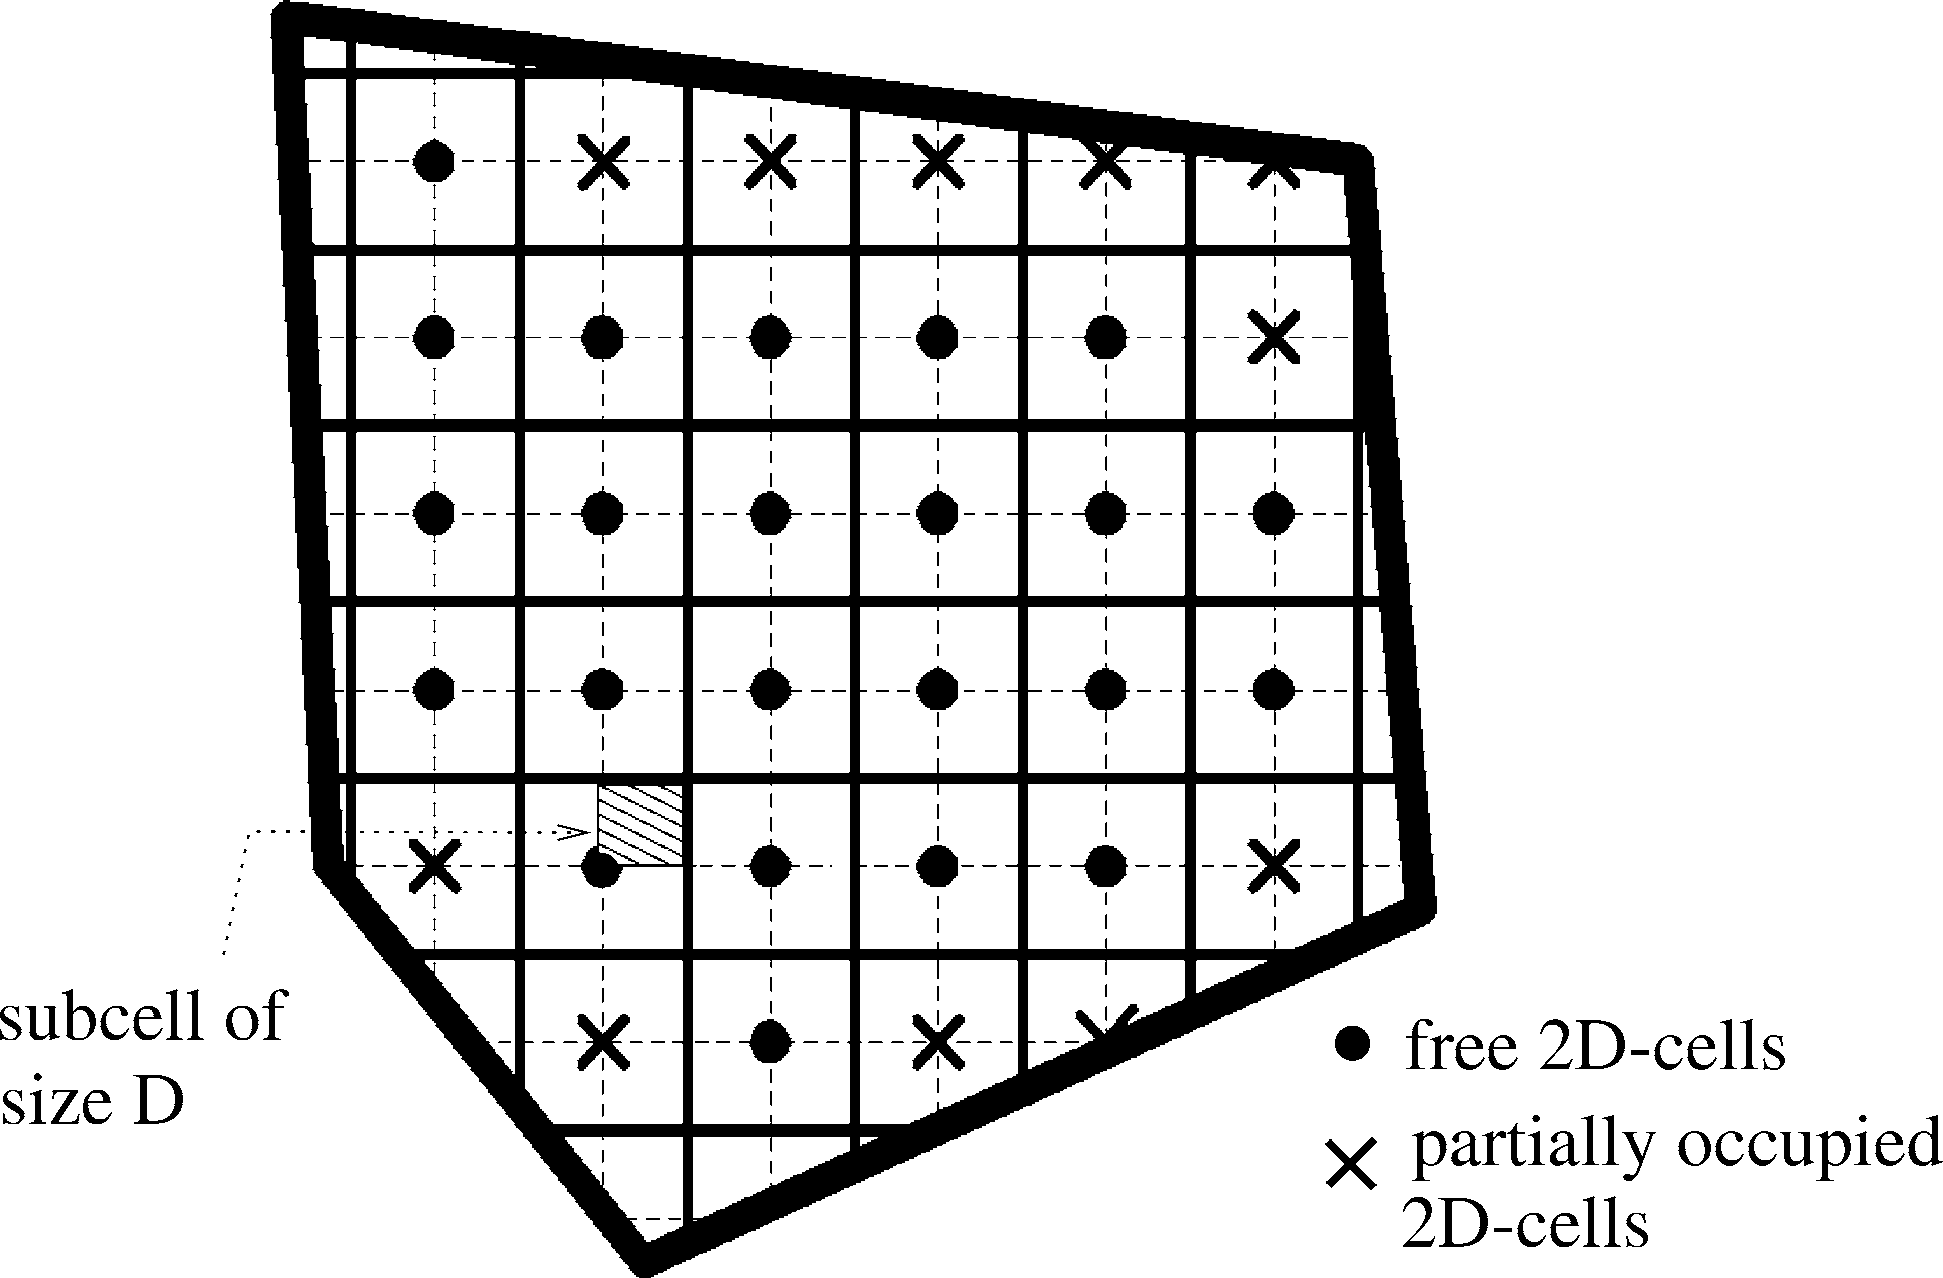
\includegraphics[width=0.8\linewidth]{Images/inv_fig1.png}
            \caption{The work-area grid}
        \end{figure}
        \column{0.5\textwidth}
        \begin{itemize}
            \item When online: robot has no apriori knowledge about environment
            \item Let $D$ be the tool size
            \item Subdivide the work-area into a grid of cells of size $D$
            \item Let $n$ be the number of free cells
            \item Obstacles are allowed
        \end{itemize}
    \end{columns}
\end{frame}

\begin{frame}{Definitions}
    \begin{columns}
        \column{0.5\textwidth}
        \begin{figure}
            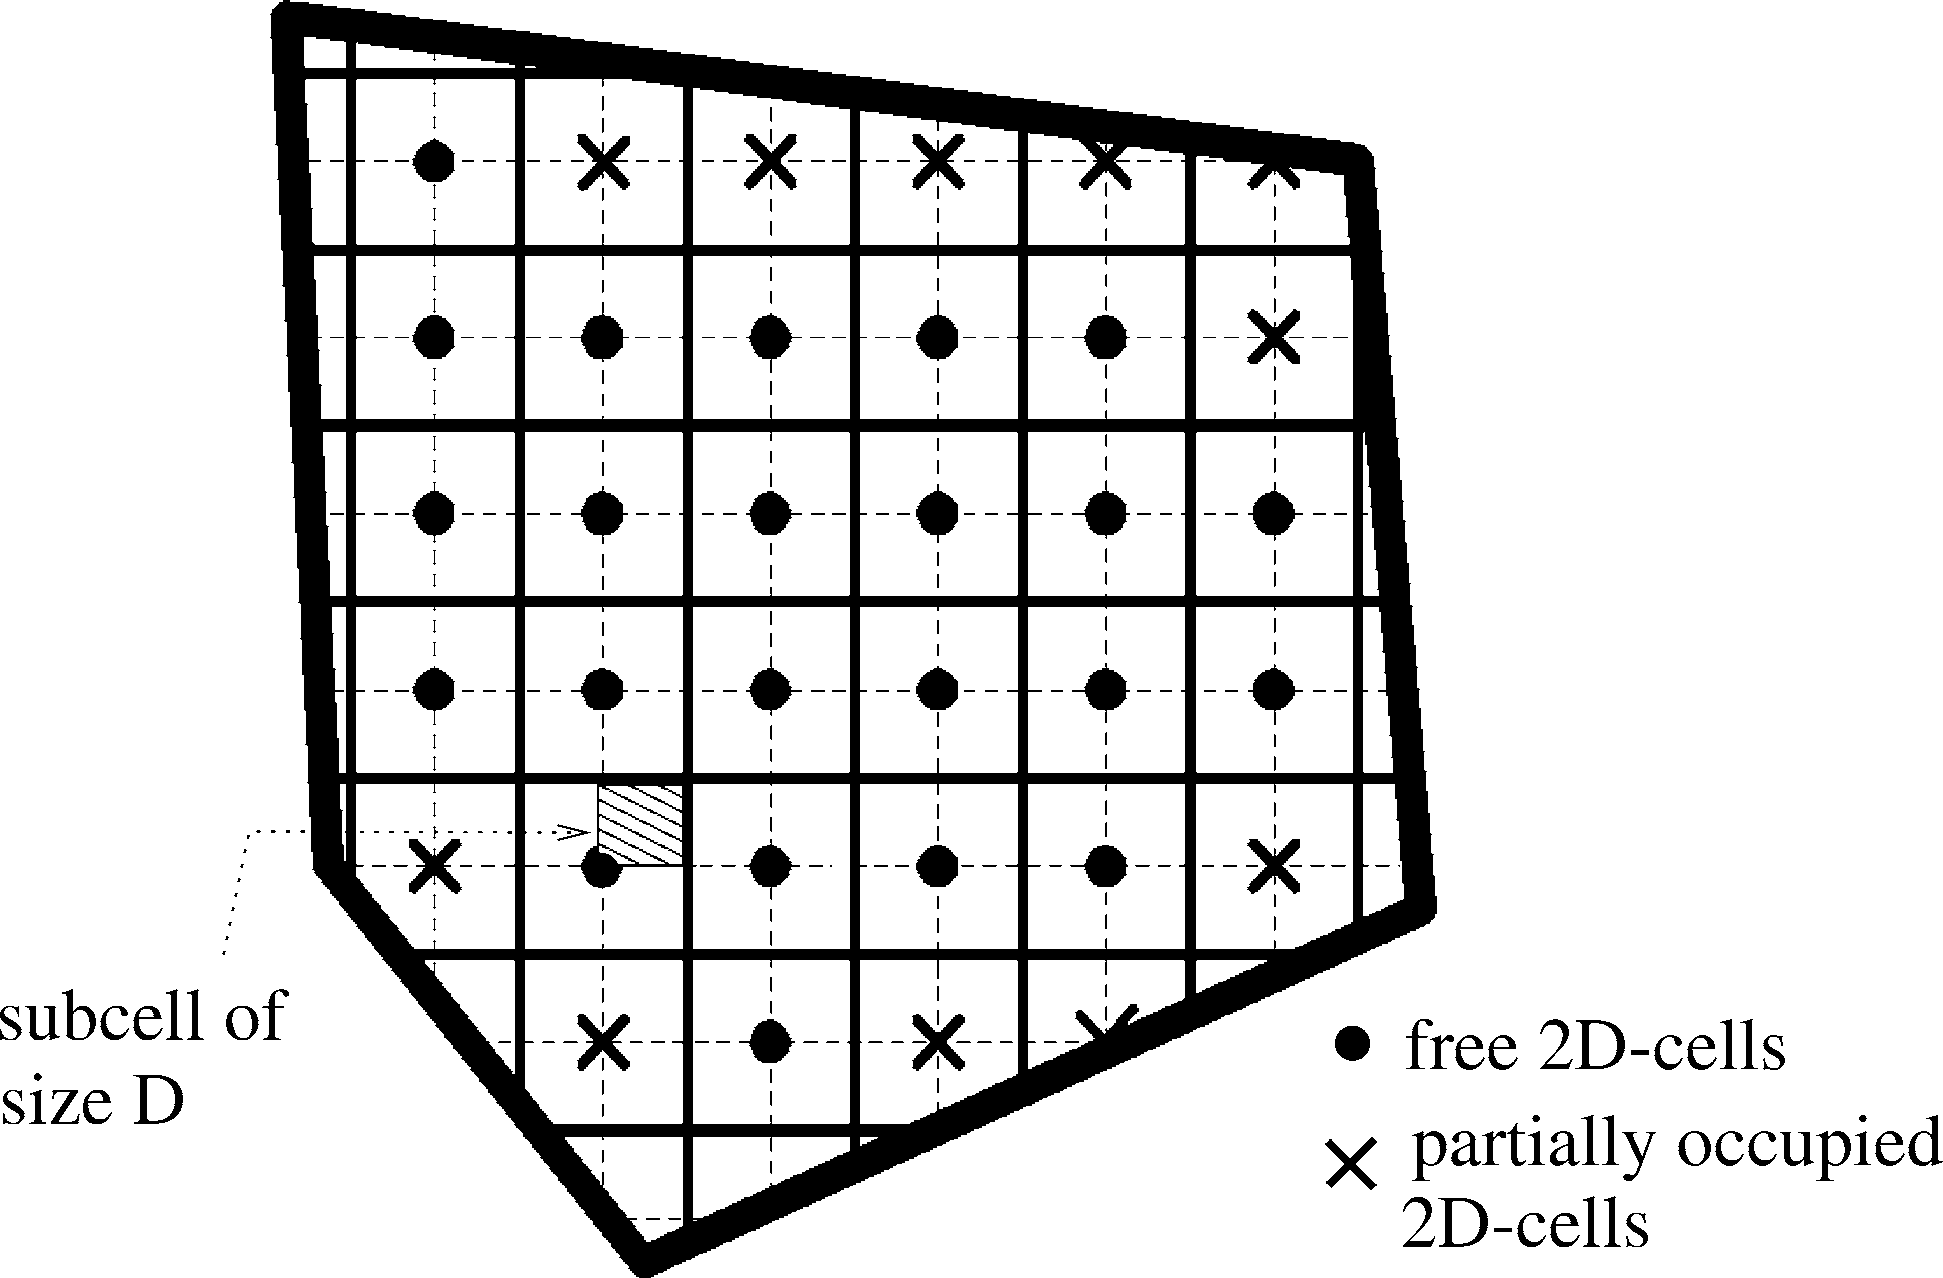
\includegraphics[width=0.8\linewidth]{Images/inv_fig1.png}
            \caption{The work-area grid}
        \end{figure}
        \column{0.5\textwidth}
        \begin{itemize}
            \item Boundary cells share at least one point with grid boundary
            \item Let $m$ be the number boundary cells
            \item Let $l_\mathcal{A}$ be the length of the path, generated by Algorithm $\mathcal{A}$
            \item $l_\mathcal{A}$ defines the cost for $\mathcal{A}$
        \end{itemize}
    \end{columns}
\end{frame}

\begin{frame}{Trivial Solution: DFS}
    \begin{columns}
        \column{0.5\textwidth}
        \begin{figure}
            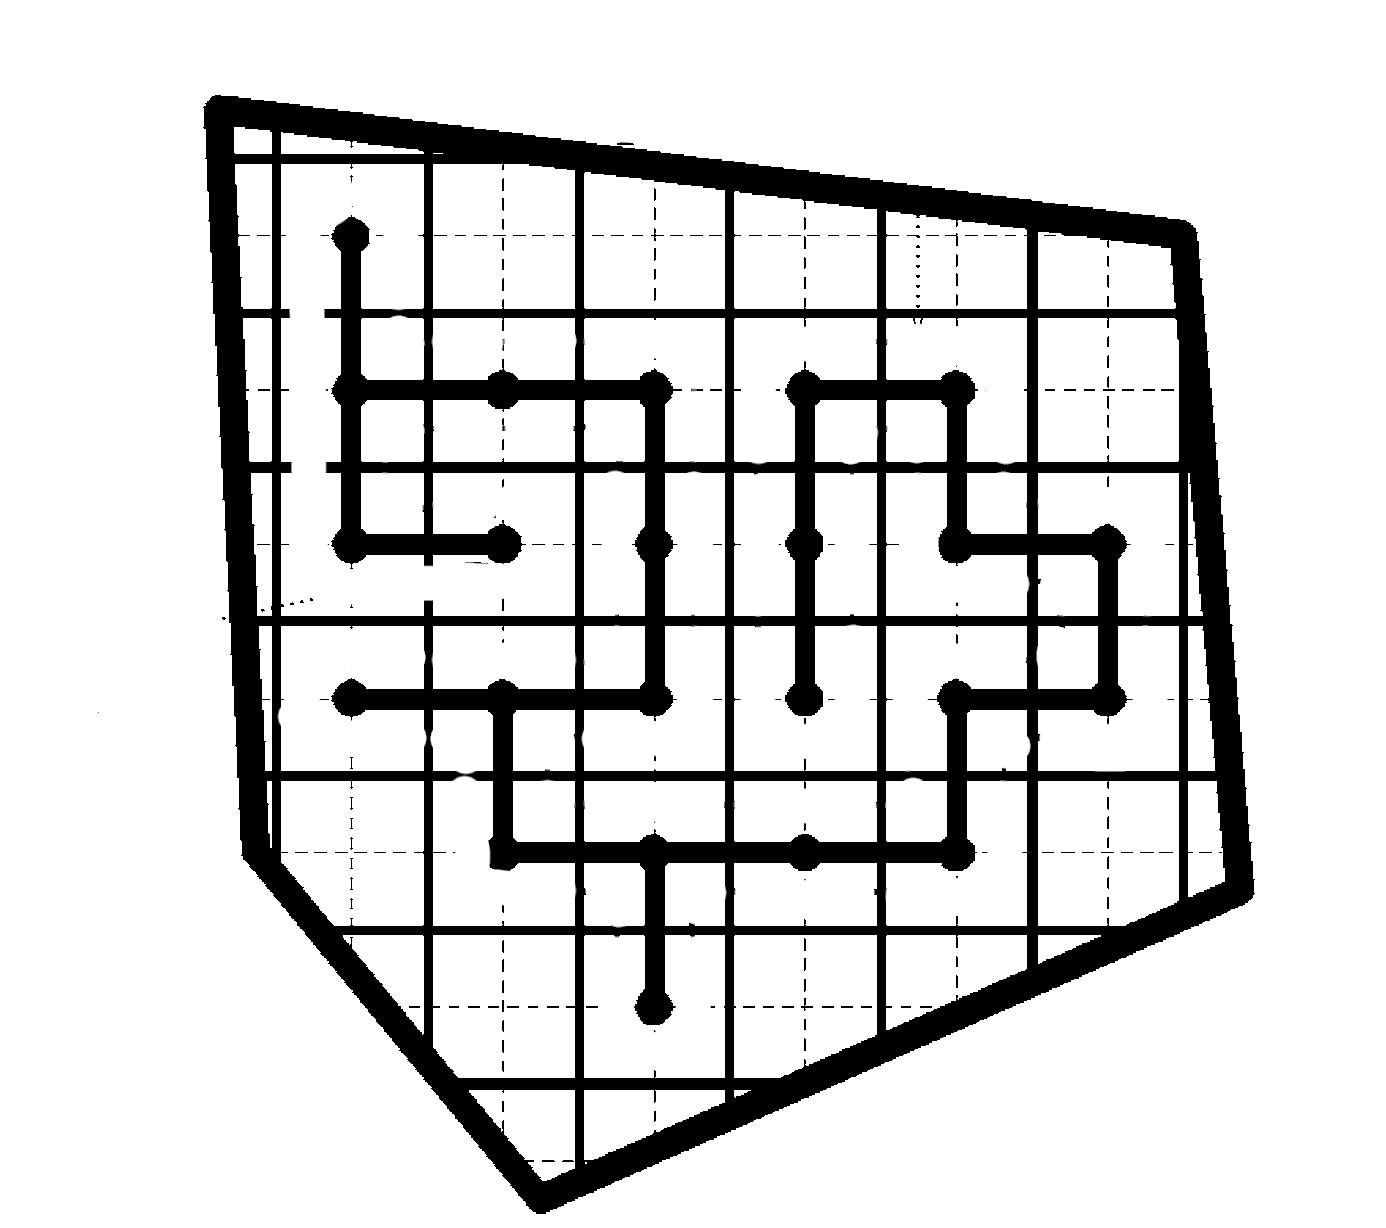
\includegraphics[width=0.8\linewidth]{Images/DFS.png}
            \caption{A trivial solution: DFS}
        \end{figure}
        \column{0.5\textwidth}
        \begin{itemize}
            \item $l_{DFS}$ is always $2nD$
            \item STC Algorithms are upper bounded by $(n + m) D$
            \item Both have comp. ratio of $2 - \epsilon$
            \item In practice $m \ll n$
        \end{itemize}
    \end{columns}
\end{frame}

% \begin{frame}{Definitions}
%     \todo[inline]{add fig1}

% \end{frame}

% \subsection{Complexity}
% \begin{frame}{Complexity}
% \end{frame}
\subsection{Related Work}
\begin{frame}{Related Work}
    \begin{itemize}
        \item 1994 Paper by Kalyanasundaram and Pruhs: Constructing competitive tours from local information
              \begin{itemize}
                  \item 16-competitive algorithm: ShortCut
              \end{itemize}
        \item 2002 On the Competitive Complexity of Navigation Tasks
              \begin{itemize}
                  \item 2-competitive algorithm: URC
              \end{itemize}
    \end{itemize}
\end{frame}

\section{Spiral STC}
\subsection{Idea}
\begin{frame}{Idea}
    \begin{itemize}
        \item Constructing minimal spanning trees online
        \item Grid of coarser 2D cells
        \item Traversal of spanning tree edges
        \item Internal covering of 2D cells
        \item Spiral-like patterns
    \end{itemize}
\end{frame}
\subsection{2D Spiral STC}
\begin{frame}{2D Spiral STC}
    \begin{block}{Recursive Function $STC1(w,x)$:}
        \begin{enumerate}
            \item Mark the current cell $x$ as an old cell.
            \item While $x$ has a new obstacle-free neighboring cell:
                  \begin{enumerate}
                      \item Scan for first \textbf{new neighbor of $x$ in ccw order}, start with parent cell $w$. Call this $y$.
                      \item Construct spanning-tree edge from $x$ to $y$.
                      \item Move to subcell of $y$ \textbf{following right-side of spanning tree edges.}
                      \item Execute STC1($x$, $y$).
                  \end{enumerate}
            \item If $x \neq S$, move back from $x$ to a subcell of $w$ \textbf{along right-side of spanning tree edges.}
        \end{enumerate}
    \end{block}
\end{frame}

\subsection{Visualization}
\begin{frame}{Visualization}
    \begin{figure}
        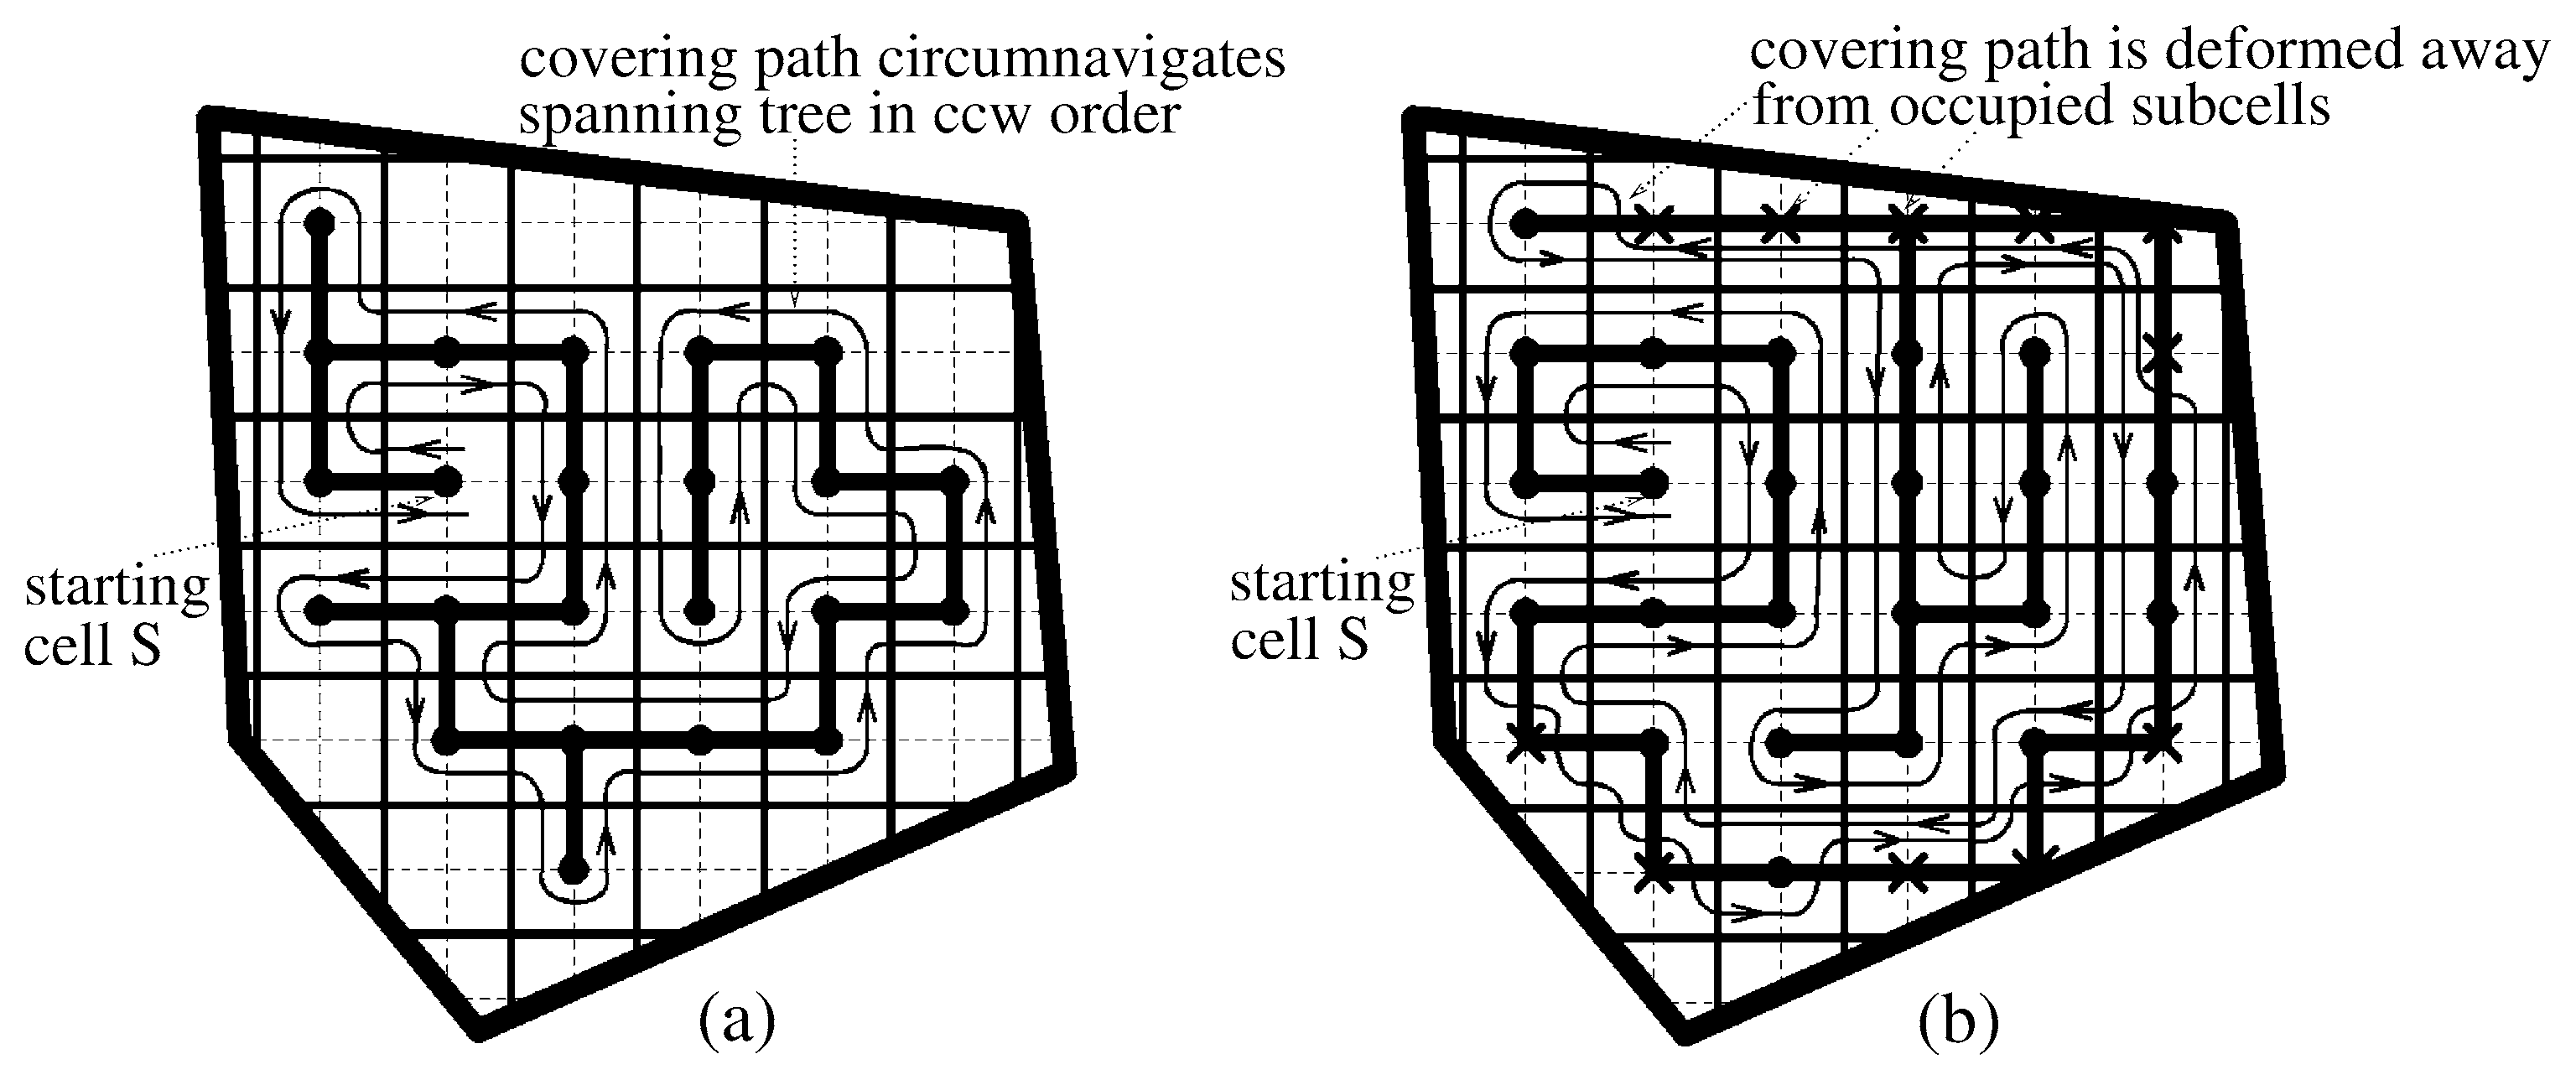
\includegraphics[width=\linewidth]{Images/inv_fig3.png}
        \caption{Visualization of the Spiral STC Algorithms}
    \end{figure}
\end{frame}

\subsection{Full Spiral STC}
\begin{frame}{Full Spiral STC}
    \begin{figure}
        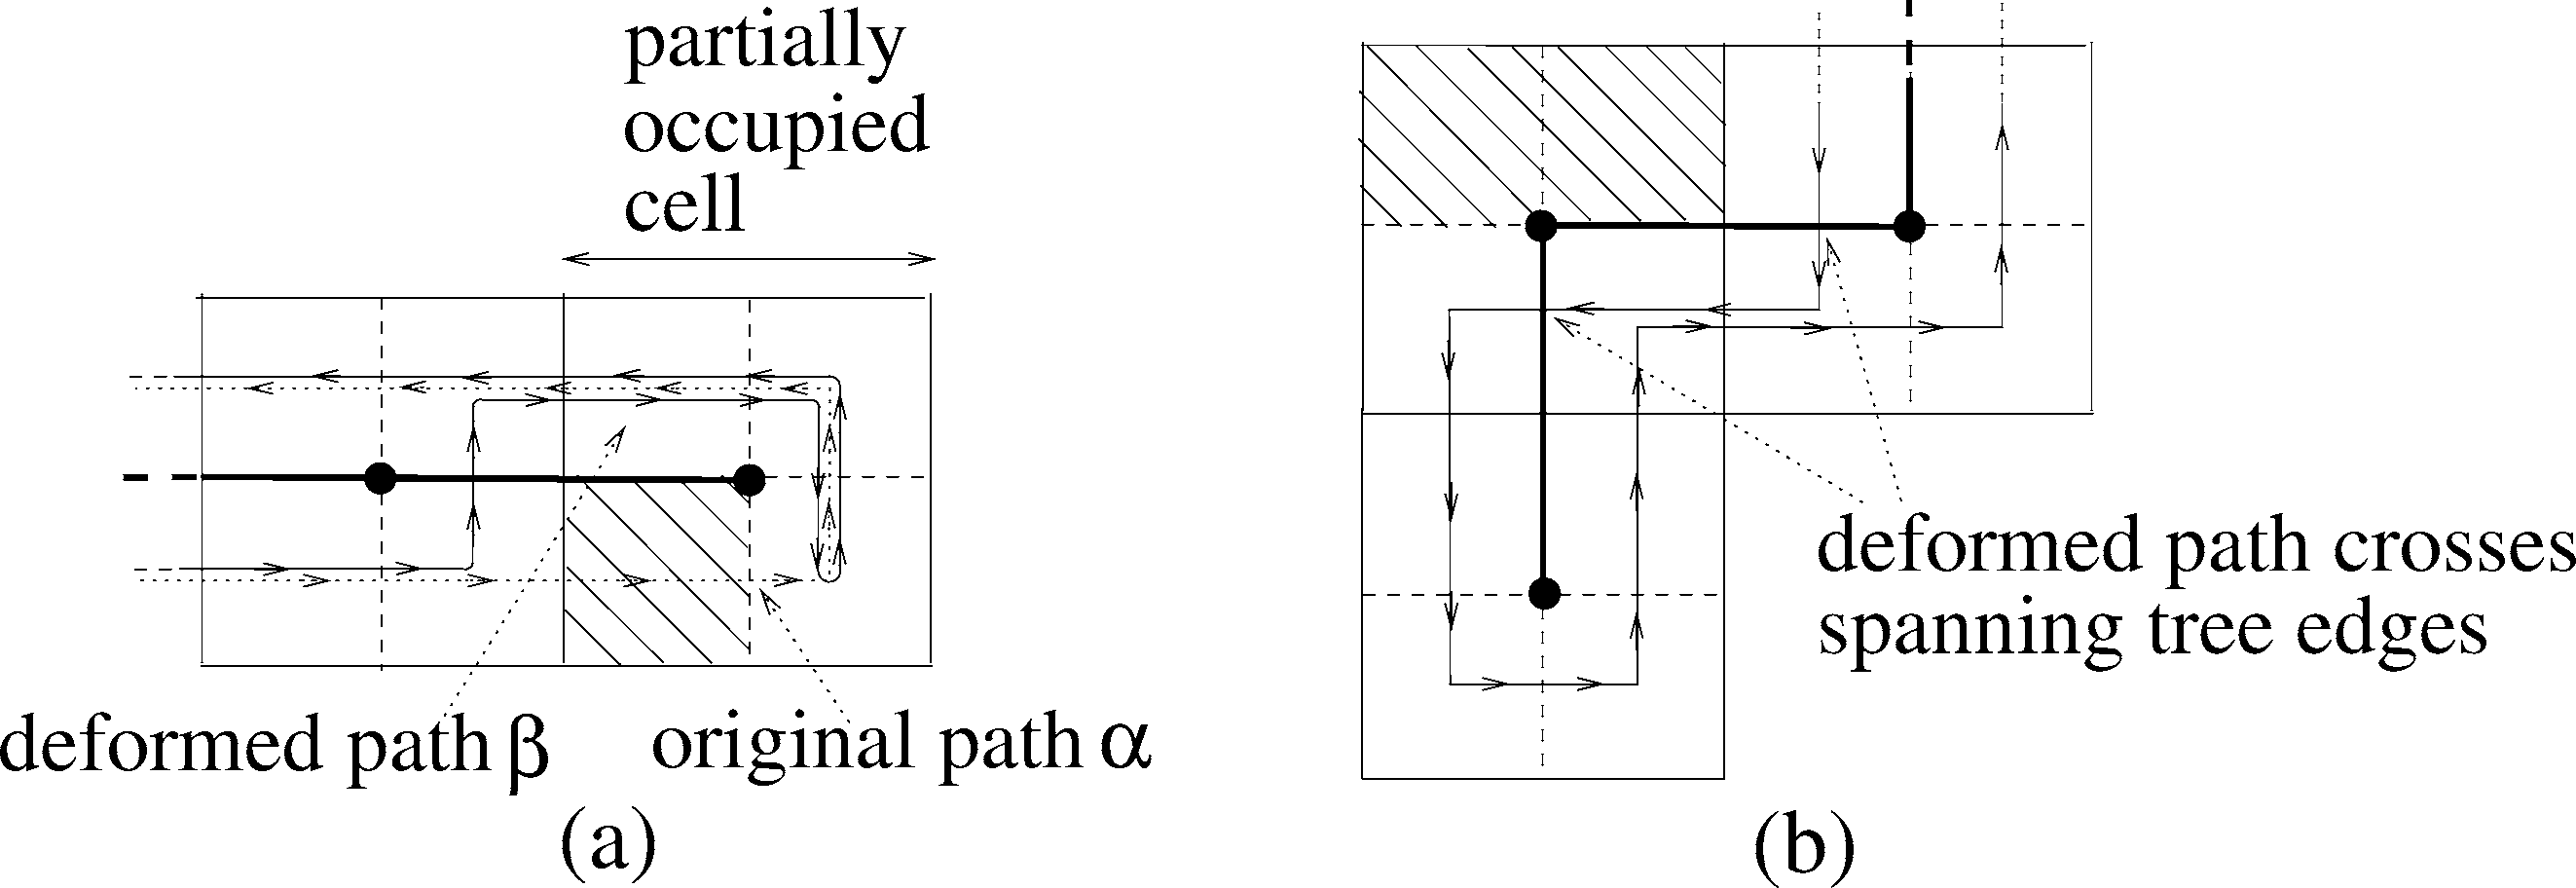
\includegraphics[width=0.8\linewidth]{Images/inv_fig5.png}
        \caption{Deforming the path to circumvent boundarys}
    \end{figure}
    \begin{itemize}
        \item Keep distance of $\frac{D}{2}$ to boundary
              % metric?
    \end{itemize}
\end{frame}

\subsection{Visualization}
\begin{frame}{Visualization}
    \begin{figure}
        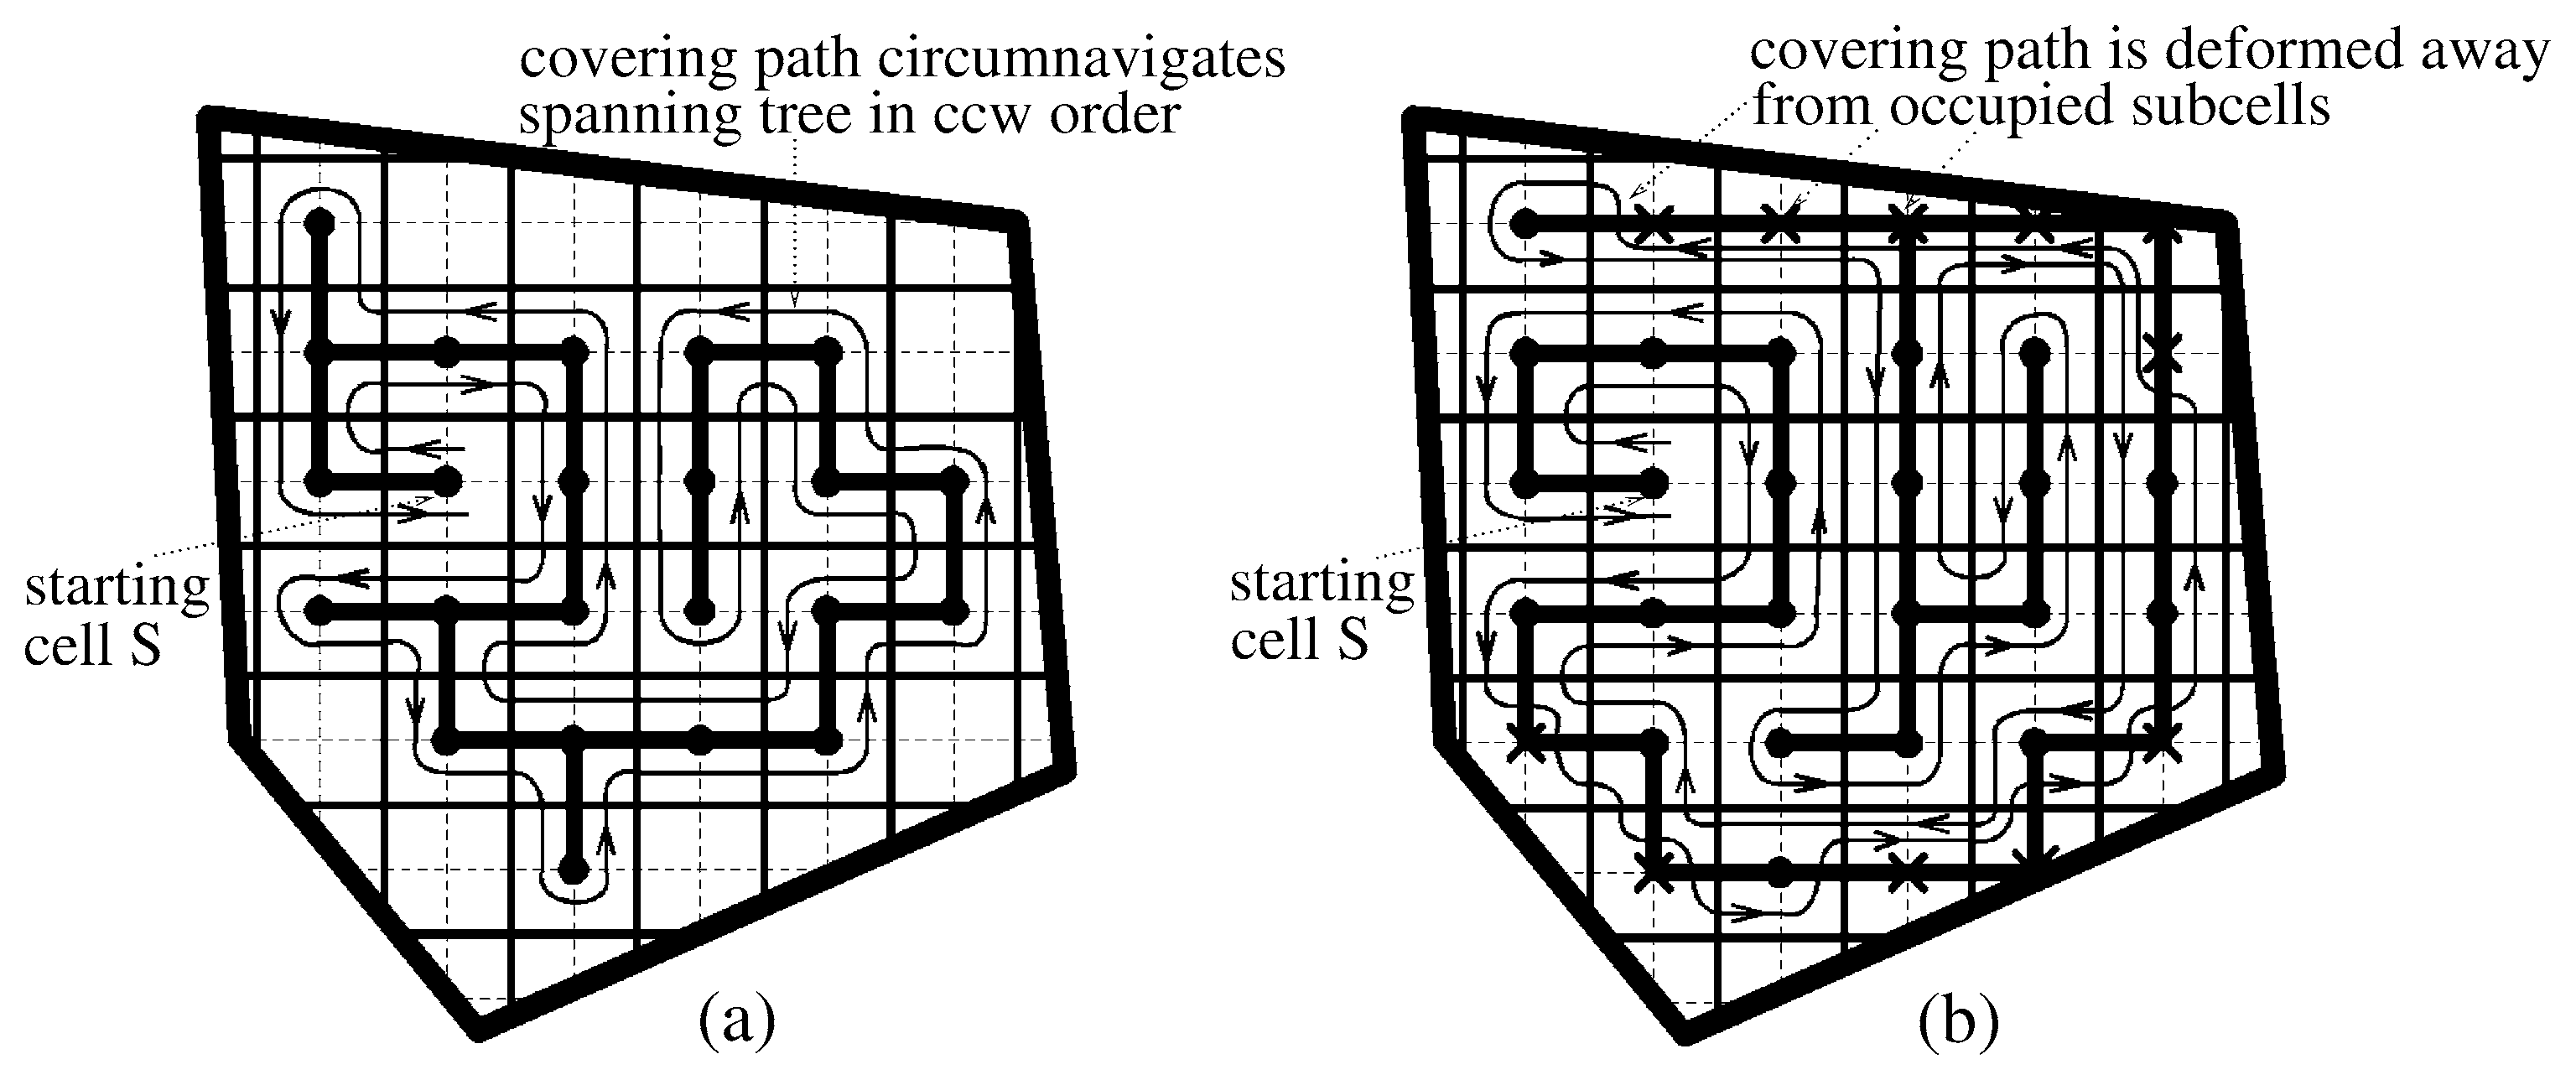
\includegraphics[width=\linewidth]{Images/inv_fig3.png}
        \caption{Visualization of the Spiral STC Algorithms}
    \end{figure}
\end{frame}

\section{Scan STC}
\subsection{Visualization}
\begin{frame}{Visualization}
    \begin{figure}
        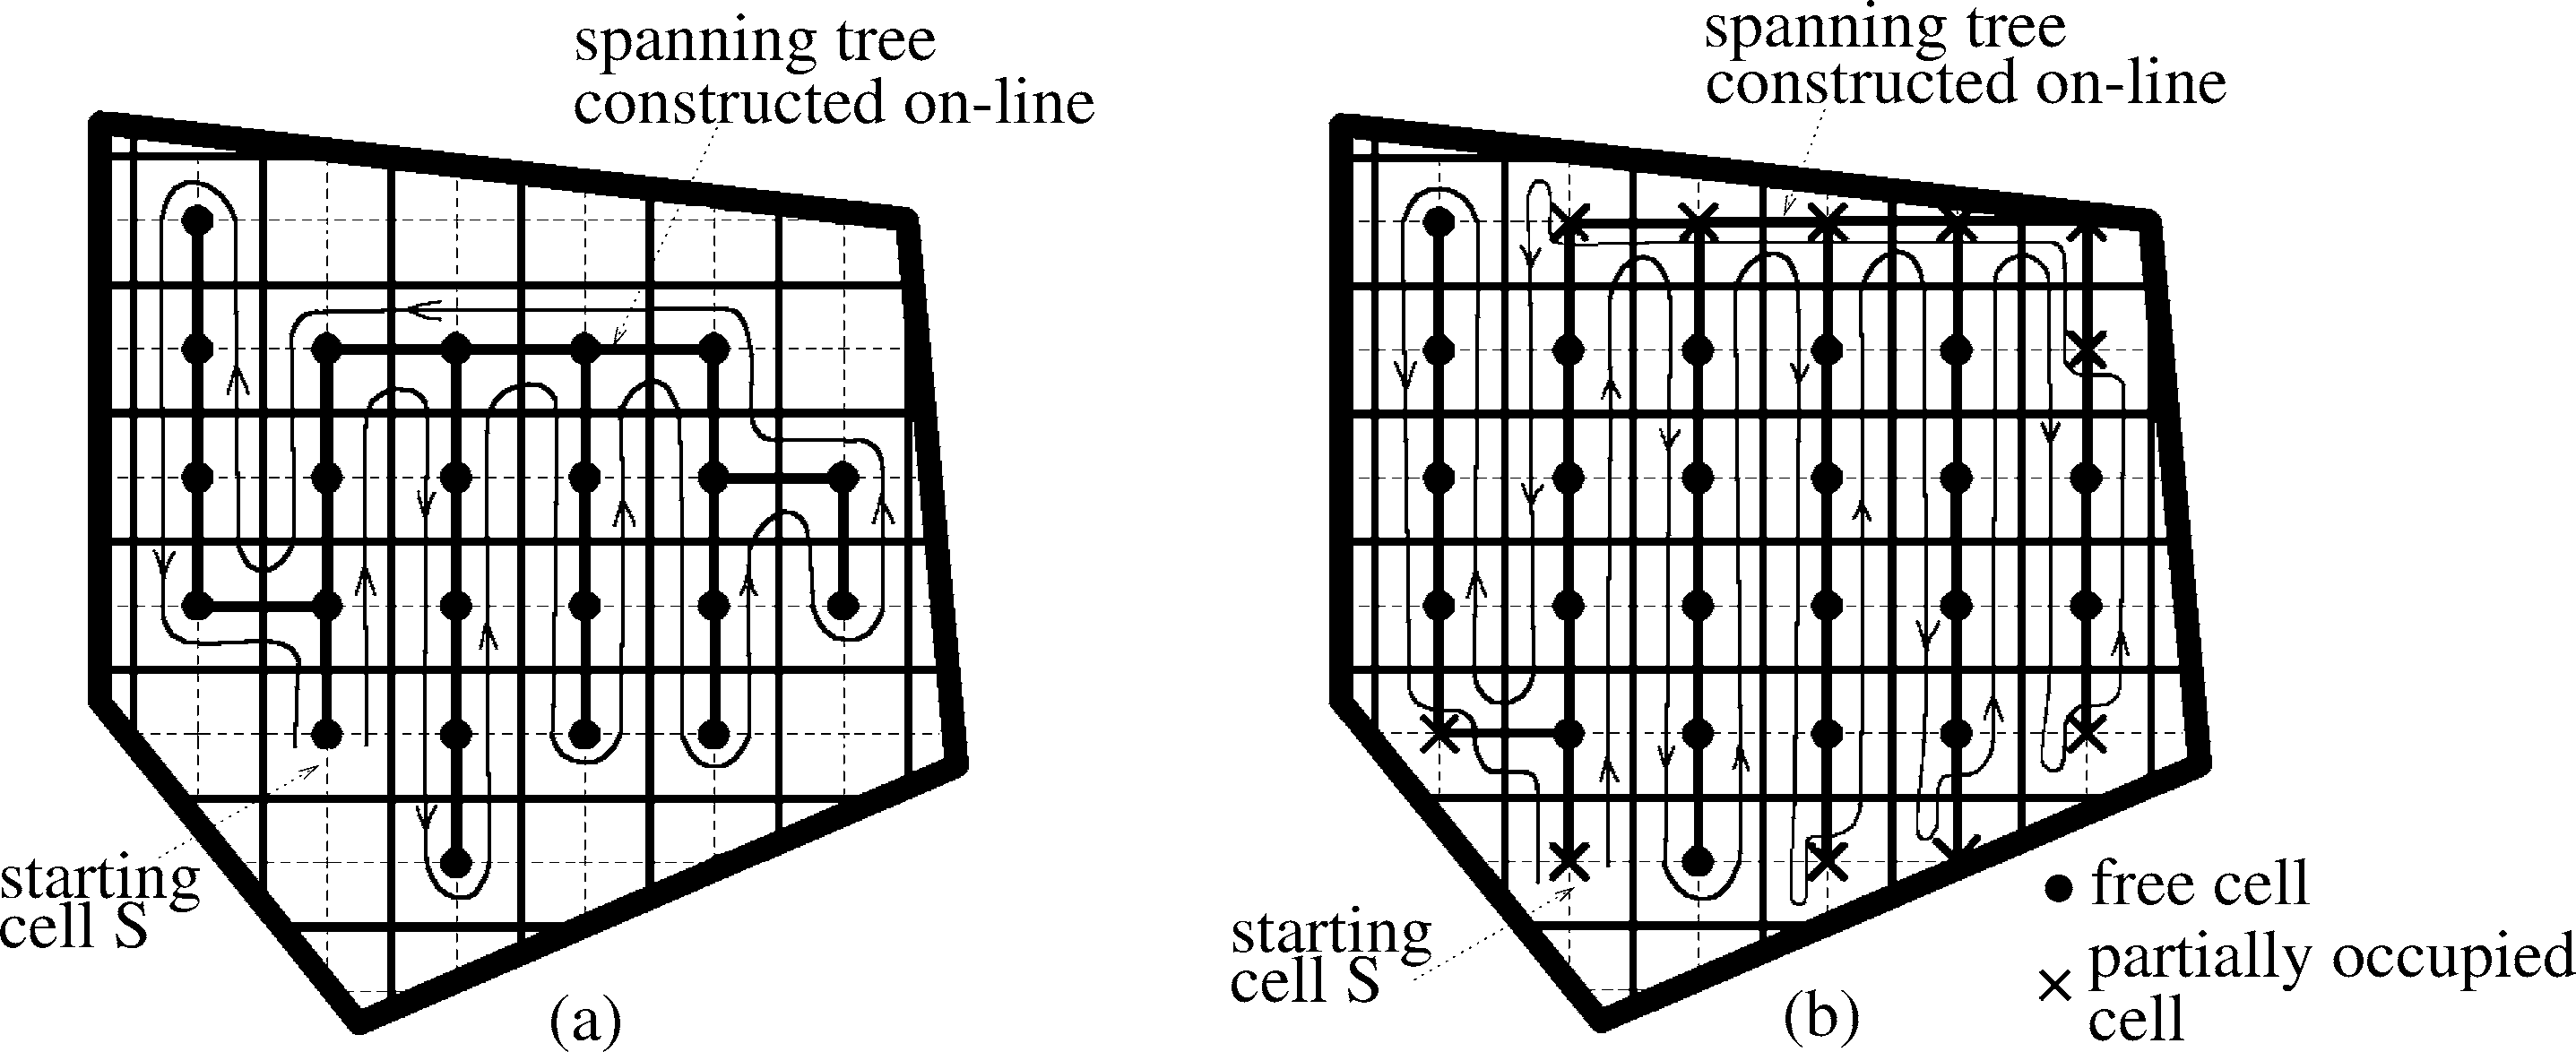
\includegraphics[width=\linewidth]{Images/inv_fig7.png}
        \caption{Visualization of the Scan STC Algorithms}
    \end{figure}
\end{frame}
\subsection{Differences to Spiral STC}
\begin{frame}{Differences to Spiral STC}
    \begin{figure}
        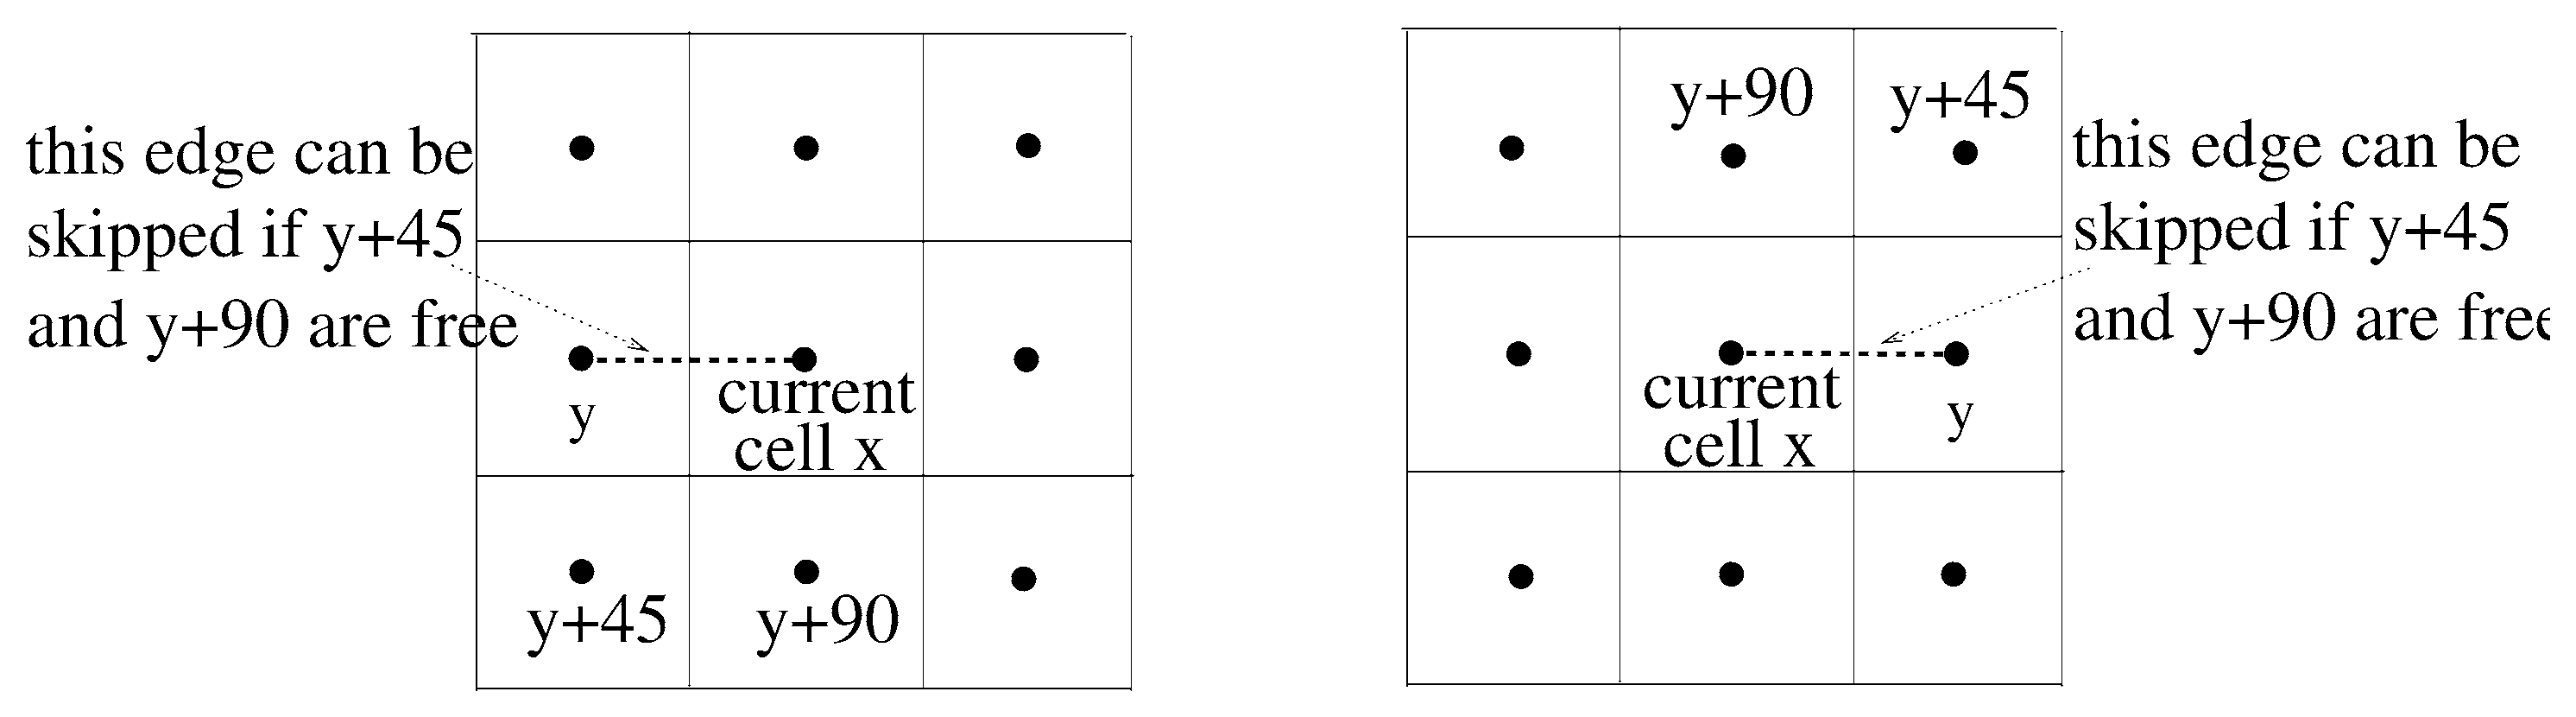
\includegraphics[width=\linewidth]{Images/inv_fig6.png}
        \caption{How Scan STC achieves scan like patterns}
    \end{figure}
\end{frame}

\section{Analysis of the Algorithms}
\subsection{Bounds}
\begin{frame}{Bounds}
    \begin{itemize}
        \item $l_{2D-STC} \leq nD$ but ignores partially occupied 2D cells
        \item $l_{Full-STC} \leq (n + m)D$
        \item STC Algorithms run in $O(n)$ time and have $O(n)$ space complexity
    \end{itemize}
    % \todo[inline]{???}
\end{frame}
\subsection{Theorem 1}
\begin{frame}{Theorem 1}
    \begin{block}{Theorem 1}
        Spiral-STC and Scan-STC cover the work-area grid using a path of total length $l \leq (n + m)D$
    \end{block}
\end{frame}
\begin{frame}{Theorem 1 - Preliminaries}
    \begin{figure}
        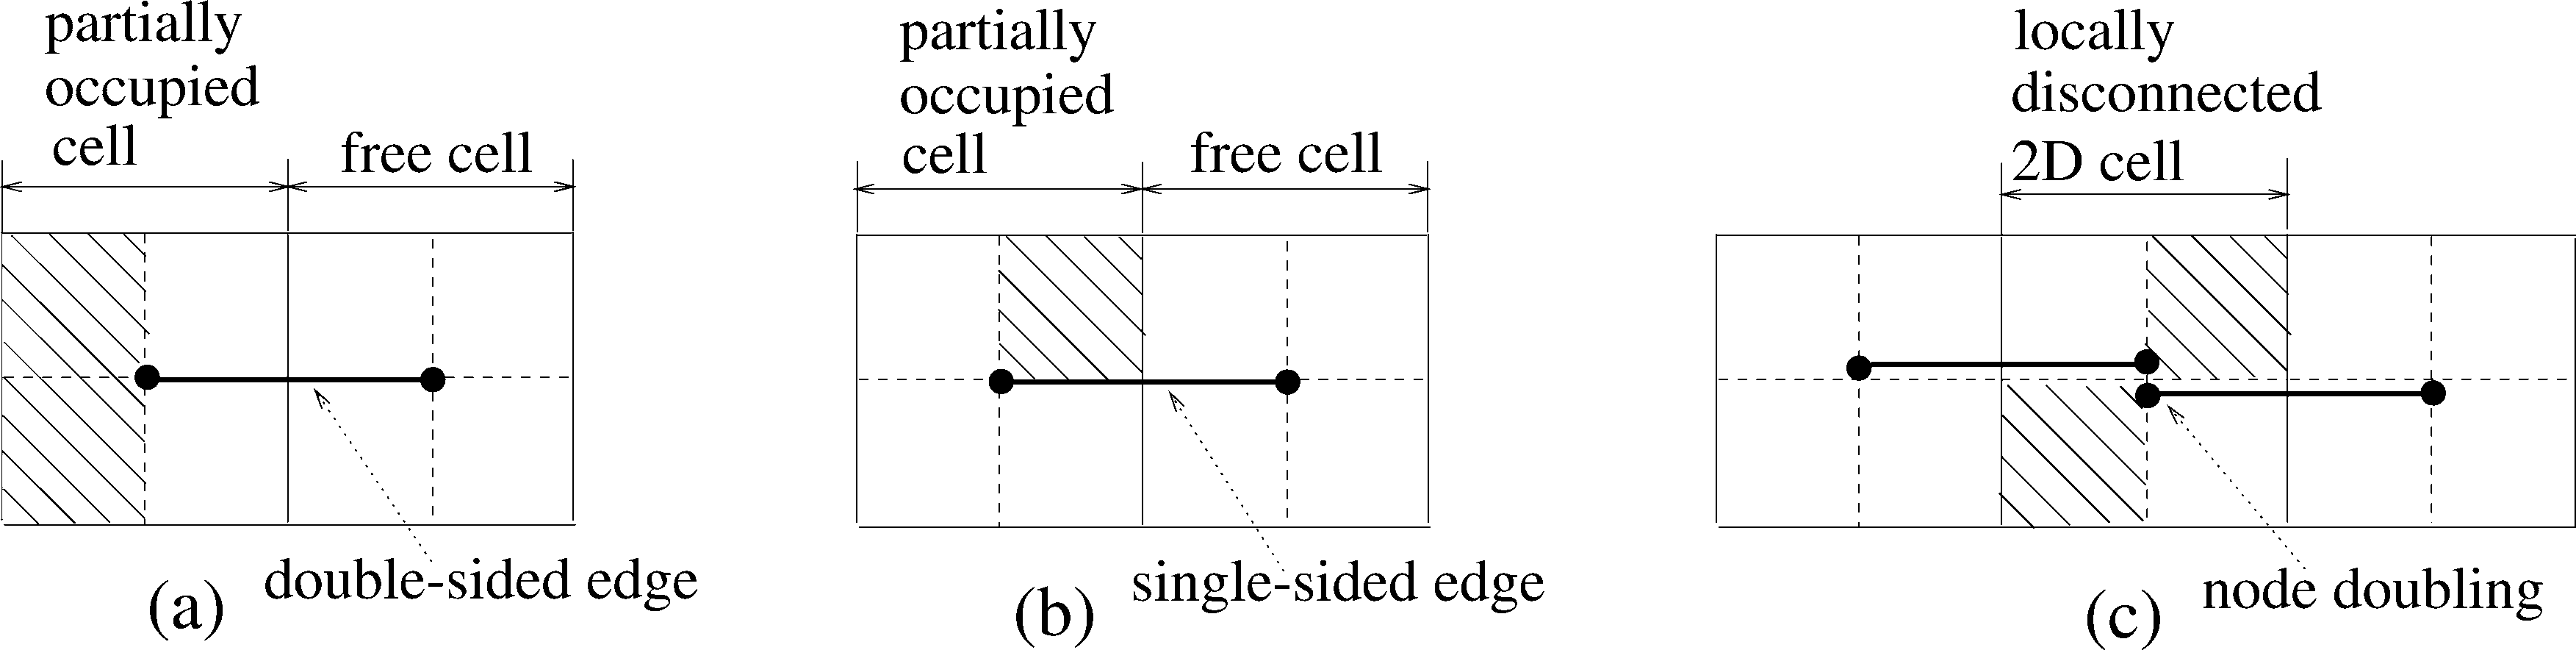
\includegraphics[width=\linewidth]{Images/inv_fig4.png}
        \caption{Single sided edges versus double sided edges.}
    \end{figure}
    \begin{itemize}
        \item Entry Edges, Exit Edges
        \item Single Sided Edge, Double Sided Edge
    \end{itemize}
\end{frame}

\begin{frame}{Theorem 1 - Preliminaries}
    \begin{itemize}
        \item Repetitive coverages
              \begin{itemize}
                  \item When a subcell is covered, then uncovered and later covered again
                  \item Inter-cell repetitive coverage: Between two 2D cells
                  \item Intra-cell repetitive coverage: Within a 2D cell
              \end{itemize}
    \end{itemize}
    \begin{figure}
        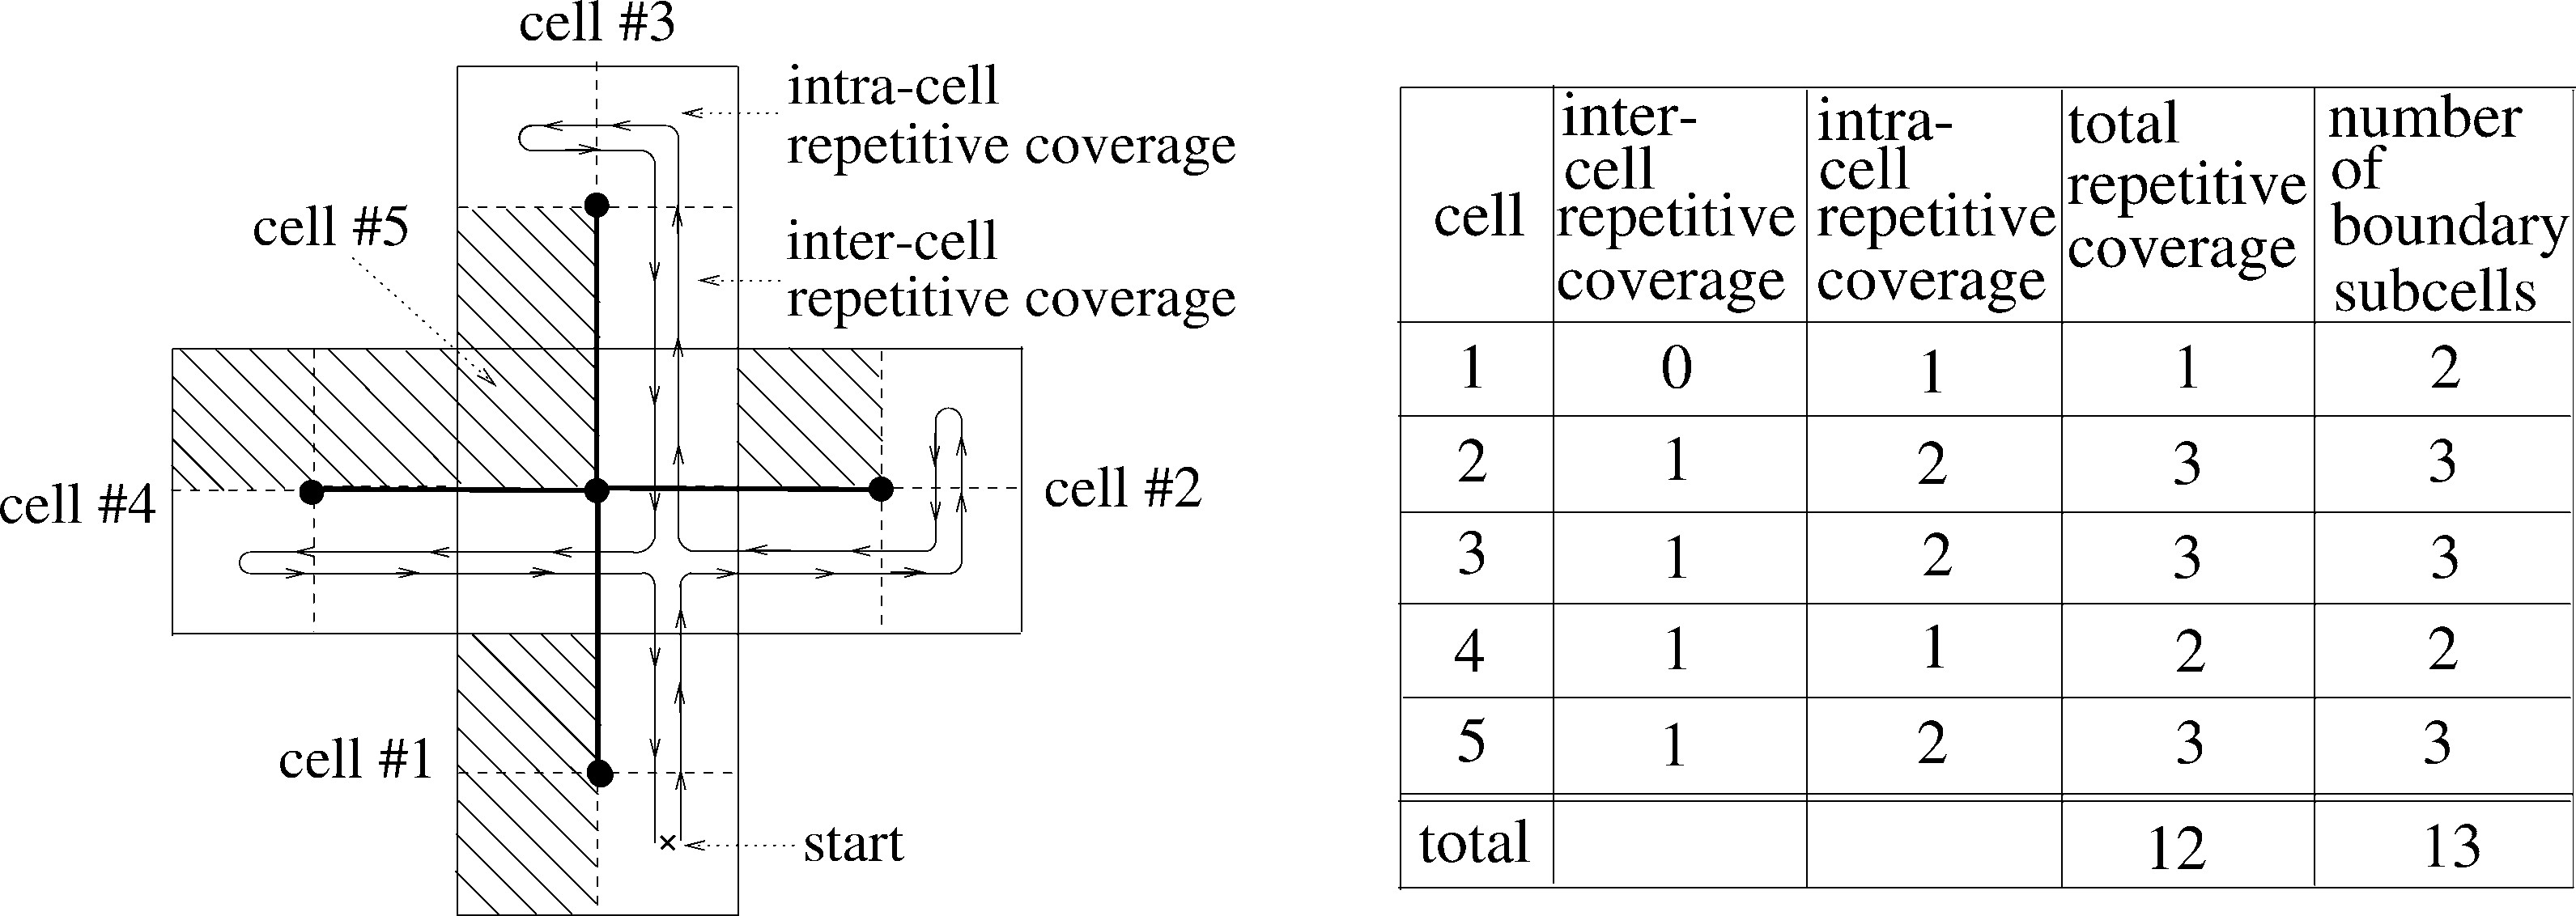
\includegraphics[width=0.8\linewidth]{Images/inv_fig9.png}
        \caption{Repetitive coverage counting of a 2D cell.}
    \end{figure}
\end{frame}

\begin{frame}{Theorem 1 - Preliminaries}
    \begin{itemize}
        \item Single sided edge $\implies$ inter-cell repetitive coverage in cell \textbf{from which it exits}
        \item Counting convention: Such rep. coverage is counted for cell \textbf{into which it enters}
        \item No change in total amount of repetitive coverages
    \end{itemize}
    \begin{figure}
        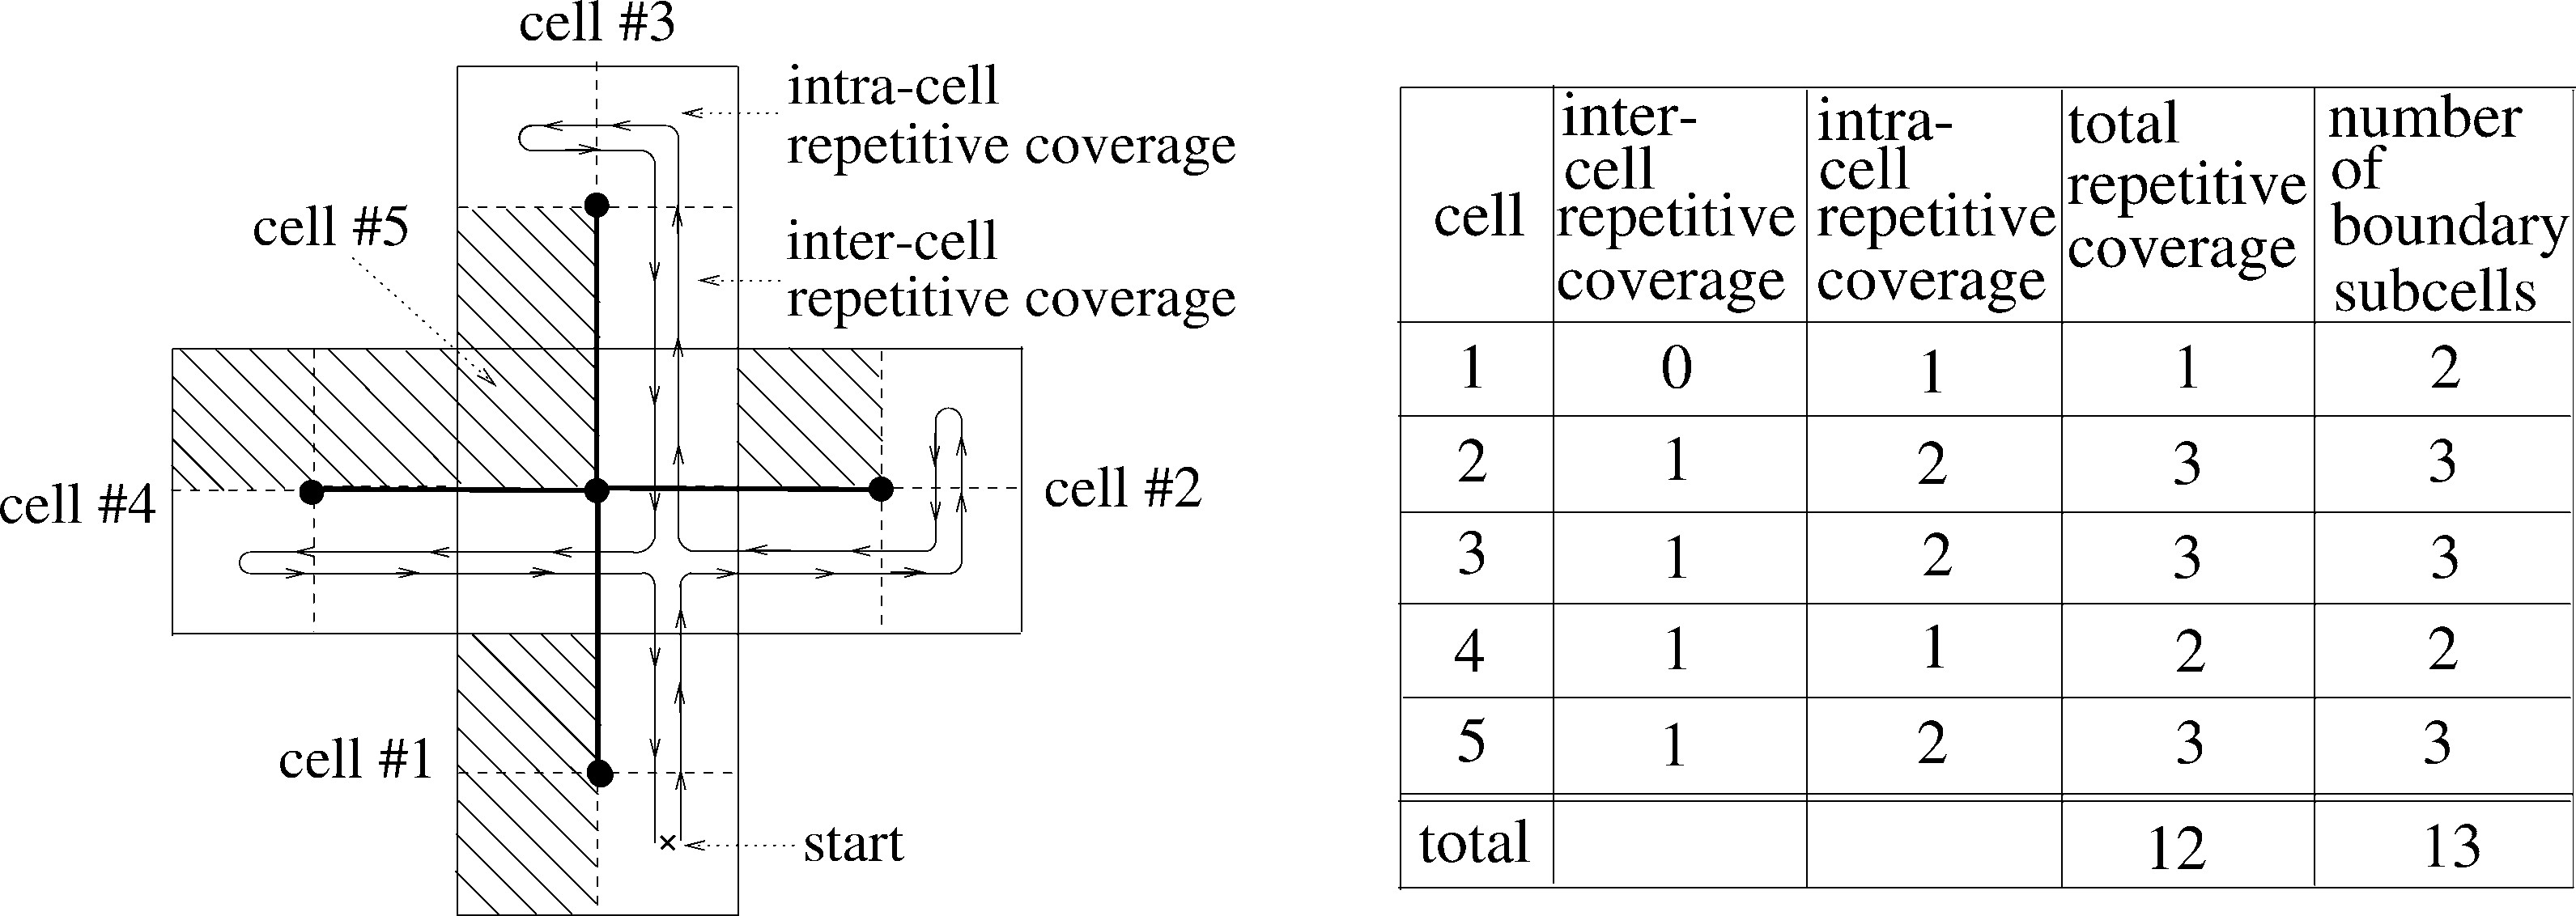
\includegraphics[width=0.8\linewidth]{Images/inv_fig9.png}
        \caption{Repetitive coverage counting of a 2D cell.}
    \end{figure}
\end{frame}


\begin{frame}{Theorem 1}
    \begin{block}{Claim 1: Total repetitive coverages bounded by $m$}
        \begin{itemize}
            \item Suffices to show for each 2D cell:

                  Total amount repetitive coverages $\leq$ Total amount of boundary cells
            \item Consider 4 cases
                  \begin{itemize}
                      \item 1 free subcell
                            \begin{itemize}
                                \item Double sided entry edge
                                \item Single sided entry edge
                            \end{itemize}
                      \item 2 free subcells
                            \begin{itemize}
                                \item Double sided entry edge
                                \item Single sided entry edge
                            \end{itemize}
                            ...
                  \end{itemize}
        \end{itemize}
    \end{block}
\end{frame}

\begin{frame}{Claim 1 - Case 1}
    \centerline{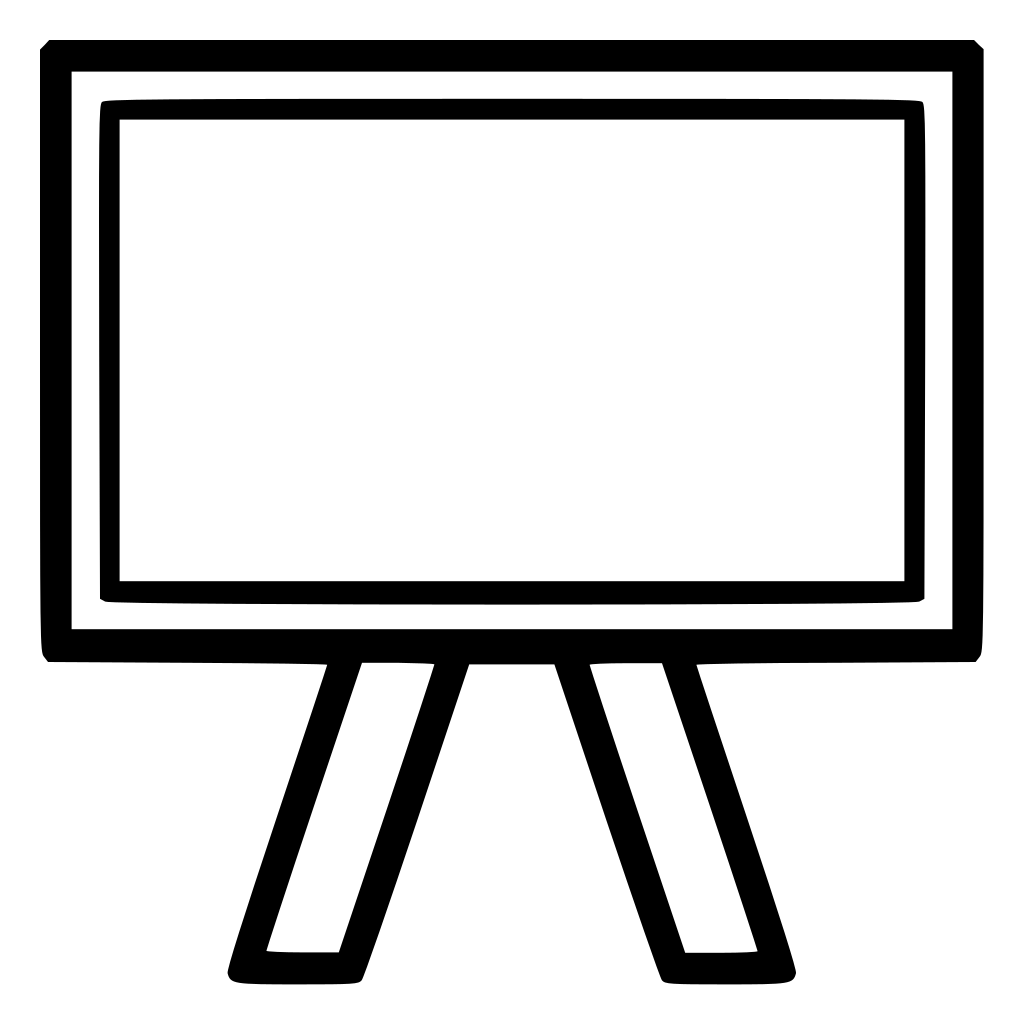
\includegraphics[width=0.2\linewidth]{Images/board.png}}
    \begin{itemize}
        \item 1 free subcell
        \item only single sided entry edge
        \item $1$ inter-cell repetitive coverage
        \item $1$ boundary cell
    \end{itemize}
\end{frame}

\begin{frame}{Claim 1 - Case 2}
    \begin{figure}
        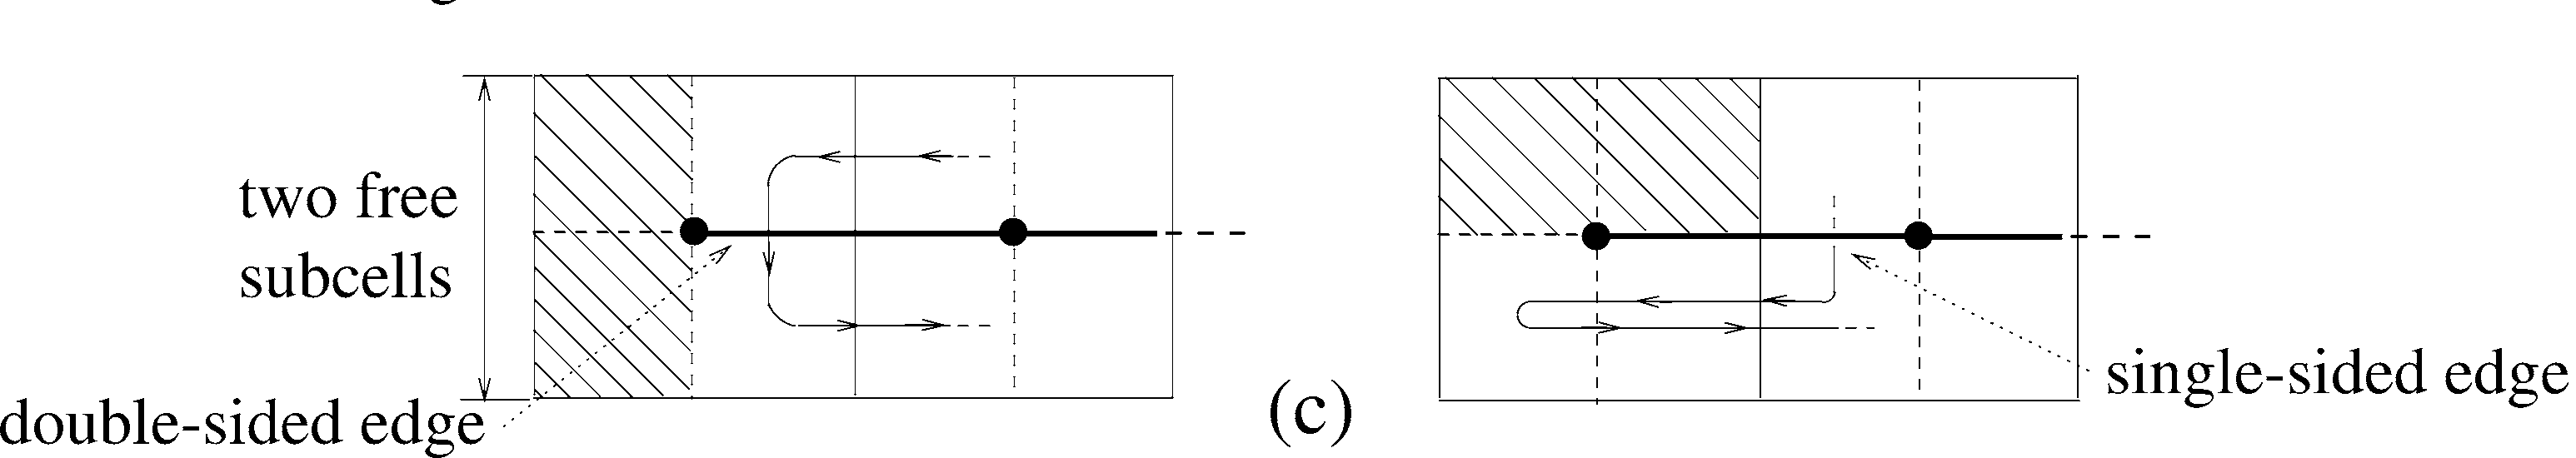
\includegraphics[width=\linewidth]{Images/inv_10_bot.png}
        \caption{2 free subcells, double sided entry edge (left) and single sided entry edge (right).}
    \end{figure}
    \todo[inline]{color boundary subcells}
    \begin{columns}
        \column{0.5\textwidth}
        \begin{itemize}
            \item $0$ repetitive coverages
            \item $2$ boundary cells
        \end{itemize}

        \column{0.5\textwidth}
        \begin{itemize}
            \item $2$ repetitive coverages
            \item $2$ boundary cells
        \end{itemize}
    \end{columns}
\end{frame}

\begin{frame}{Claim 1 - Case 3}
    \begin{figure}
        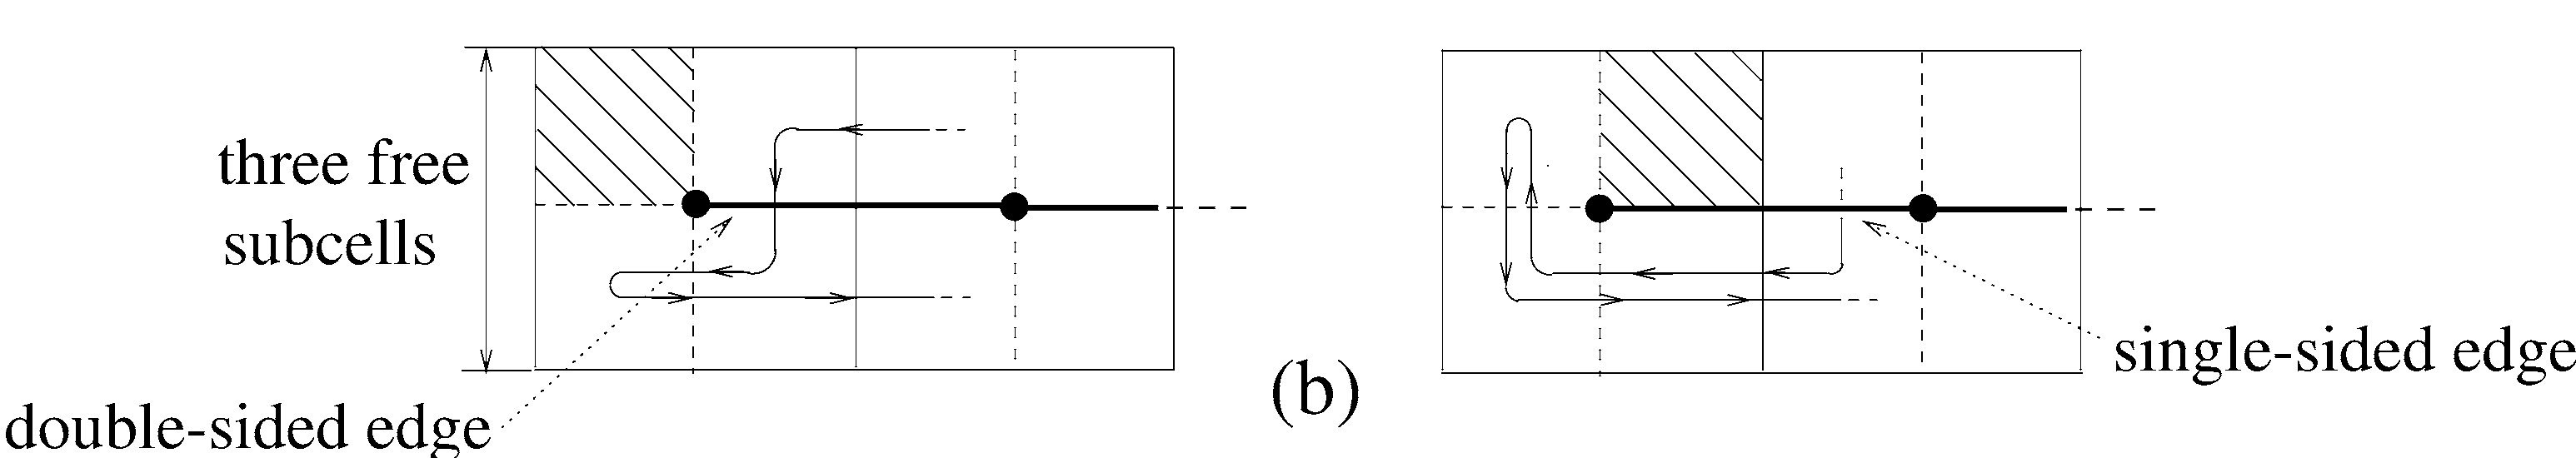
\includegraphics[width=\linewidth]{Images/inv_10_mid.png}
        \caption{3 free subcells, double sided entry edge (left) and single sided entry edge (right).}
    \end{figure}
    \begin{columns}
        \column{0.5\textwidth}
        \begin{itemize}
            \item $1$ repetitive coverages
            \item $3$ boundary cells
        \end{itemize}

        \column{0.5\textwidth}
        \begin{itemize}
            \item $3$ repetitive coverages
            \item $3$ boundary cells
        \end{itemize}
    \end{columns}
\end{frame}

\begin{frame}{Claim 1 - Case 4}
    \begin{figure}
        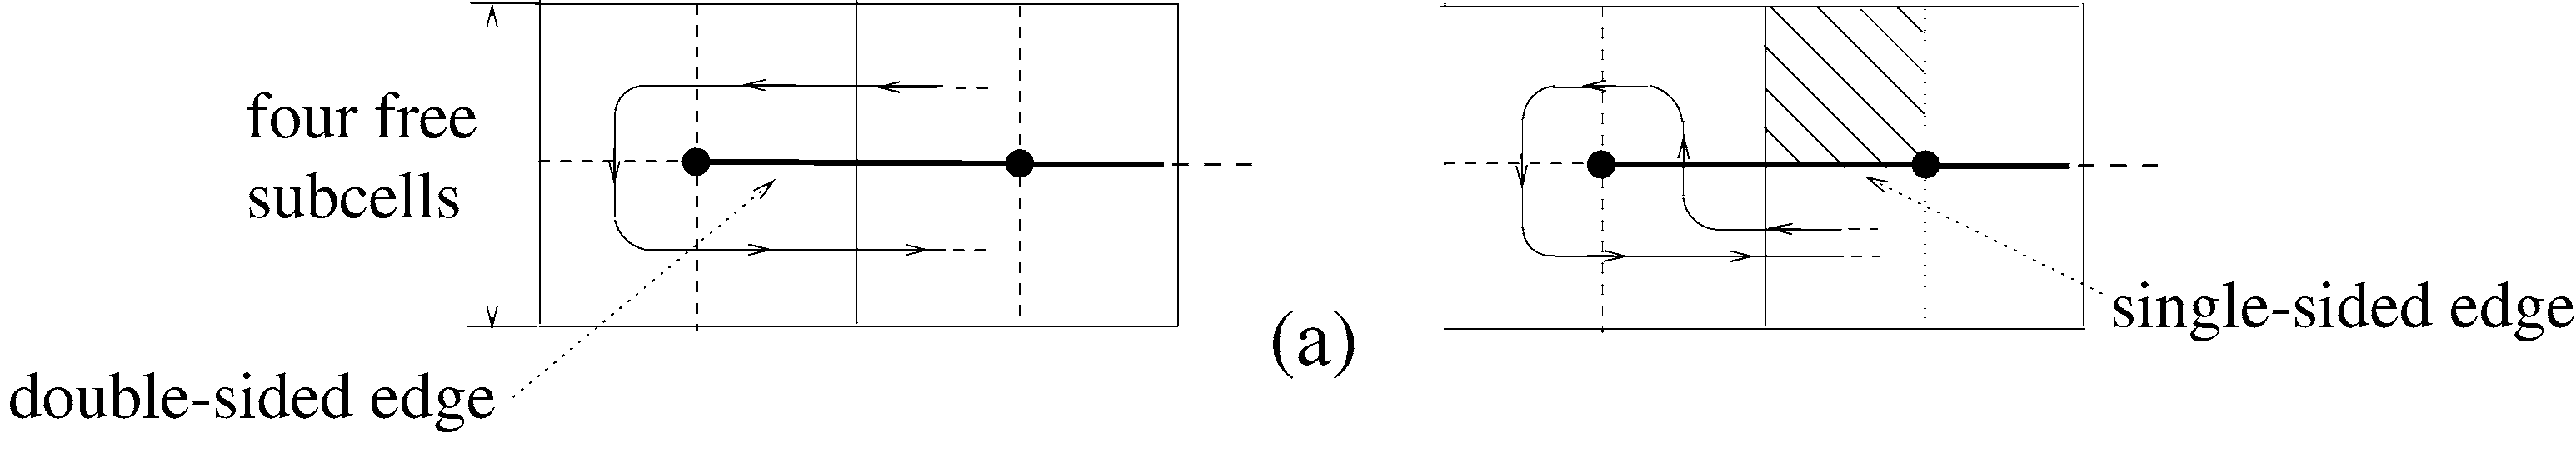
\includegraphics[width=\linewidth]{Images/inv_10_top.png}
        \caption{4 free subcells, double sided entry edge (left) and single sided entry edge (right).}
    \end{figure}
    \begin{columns}
        \column{0.5\textwidth}
        \begin{itemize}
            \item No repetitive coverages
            \item No boundary cells
        \end{itemize}

        \column{0.5\textwidth}
        \begin{itemize}
            \item $2$ repetitive coverages
            \item $2$ boundary cells
        \end{itemize}
    \end{columns}
\end{frame}
\begin{frame}{Claim 1}
    \begin{proof}
        Claim 1: Total repetitive coverages bounded by $m$
        \begin{itemize}
            \item Suffices to show for each 2D cell:

                  Total amount repetitive coverages $\leq$ Total amount of boundary cells
            \item Consider 4 cases
                  \begin{itemize}
                      \item ...
                      \item 3 free subcells
                            \begin{itemize}
                                \item Double sided entry edge
                                \item Single sided entry edge
                            \end{itemize}
                      \item 4 free subcells
                            \begin{itemize}
                                \item Double sided entry edge
                                \item Single sided entry edge
                            \end{itemize}
                  \end{itemize}
        \end{itemize}
    \end{proof}
\end{frame}

\begin{frame}{Theorem 1}
    \begin{proof}
        \begin{itemize}
            \item Every cell covered at least once: $n$
            \item (Claim 1) Number of repetitive coverages is at most $m$
            \item $\implies l_{STC} \leq (n+m) D$
        \end{itemize}
    \end{proof}
\end{frame}

\subsection{Optimality and Competitive Ratio}
\begin{frame}{Optimality and Competitive Ratio}
    \begin{itemize}
        \item Area of grid: $A := n \cdot D^2$
        \item Area of boundary cells: $\delta A := m \cdot D^2$
        \item $l_{opt} \geq \frac{A}{D} = \frac{nD^2}{D} = n \cdot D$
        \item $l_{stc} \leq (n + m) \cdot D$
    \end{itemize}

    $$ \frac{l_{stc}}{l_{opt}} \leq \frac{(n+m) \cdot D}{n \cdot D} = ... = 1 + \frac{mD^2}{nD^2} = 1 + \frac{\delta A}{A} = 2 - \epsilon$$
    with $\epsilon = (1 - \frac{\delta A}{A})$ and $0 \leq \epsilon \leq 1$ as $A \geq \delta A$ and $A, \delta A \geq 0$
\end{frame}

\section{Universal Lower Bound}
\begin{frame}{Universal Lower Bound}
    \begin{figure}
        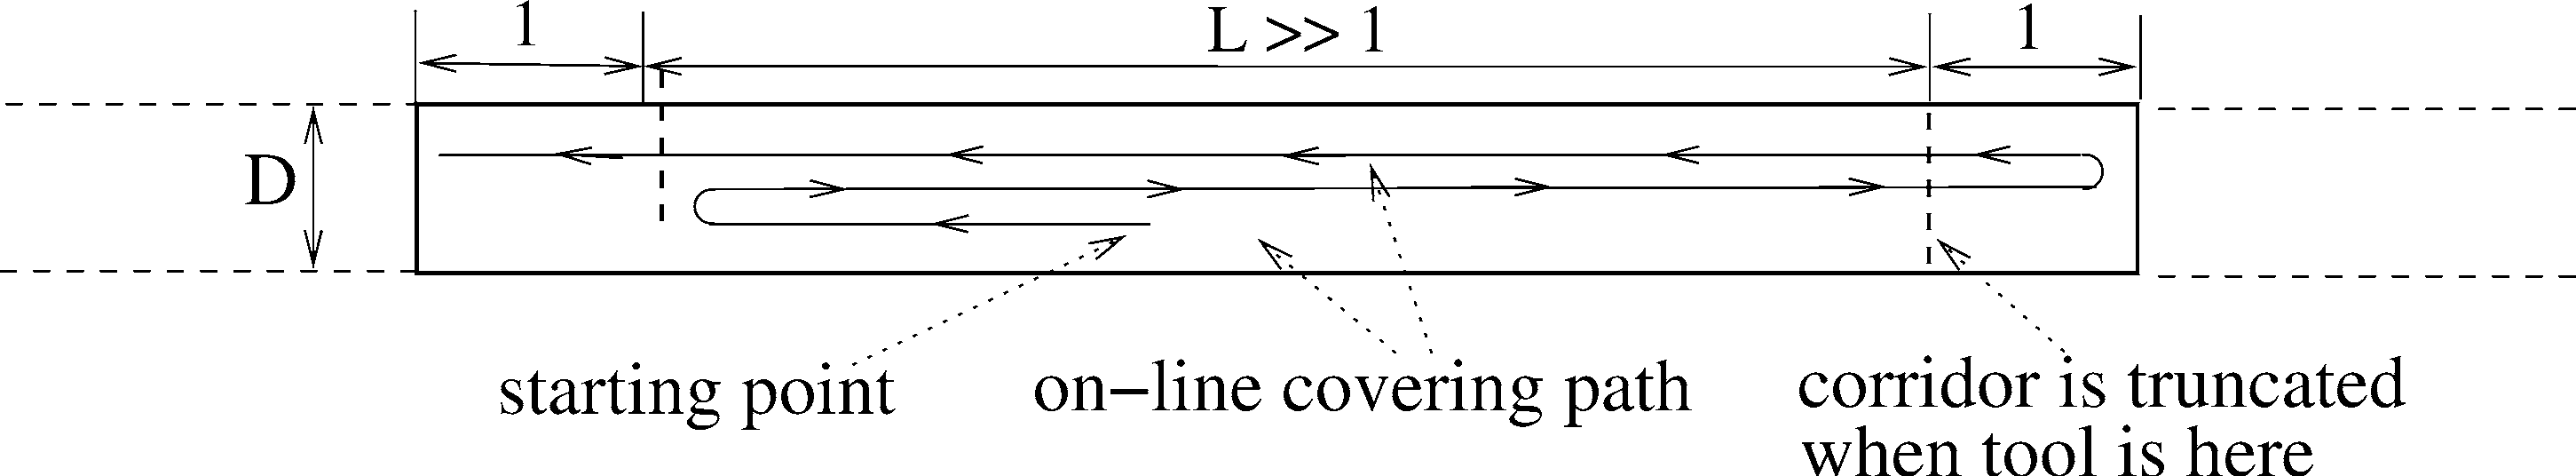
\includegraphics[width=\linewidth]{Images/inv_fig12.png}
        \caption{Trivial corridor example.}
    \end{figure}
    \begin{itemize}
        \item Simple Corridor with width $D$
        \item Corridor truncated when $L$ portion is covered
        \item $l \geq 2L + 3$
        \item $l_{opt} = L + 2$
        \item Does not show bounds for tour req.
        \item Different starting positions
    \end{itemize}
\end{frame}
\begin{frame}{Theorem 2}
    \begin{columns}
        \column{0.5\textwidth}
        \begin{figure}
            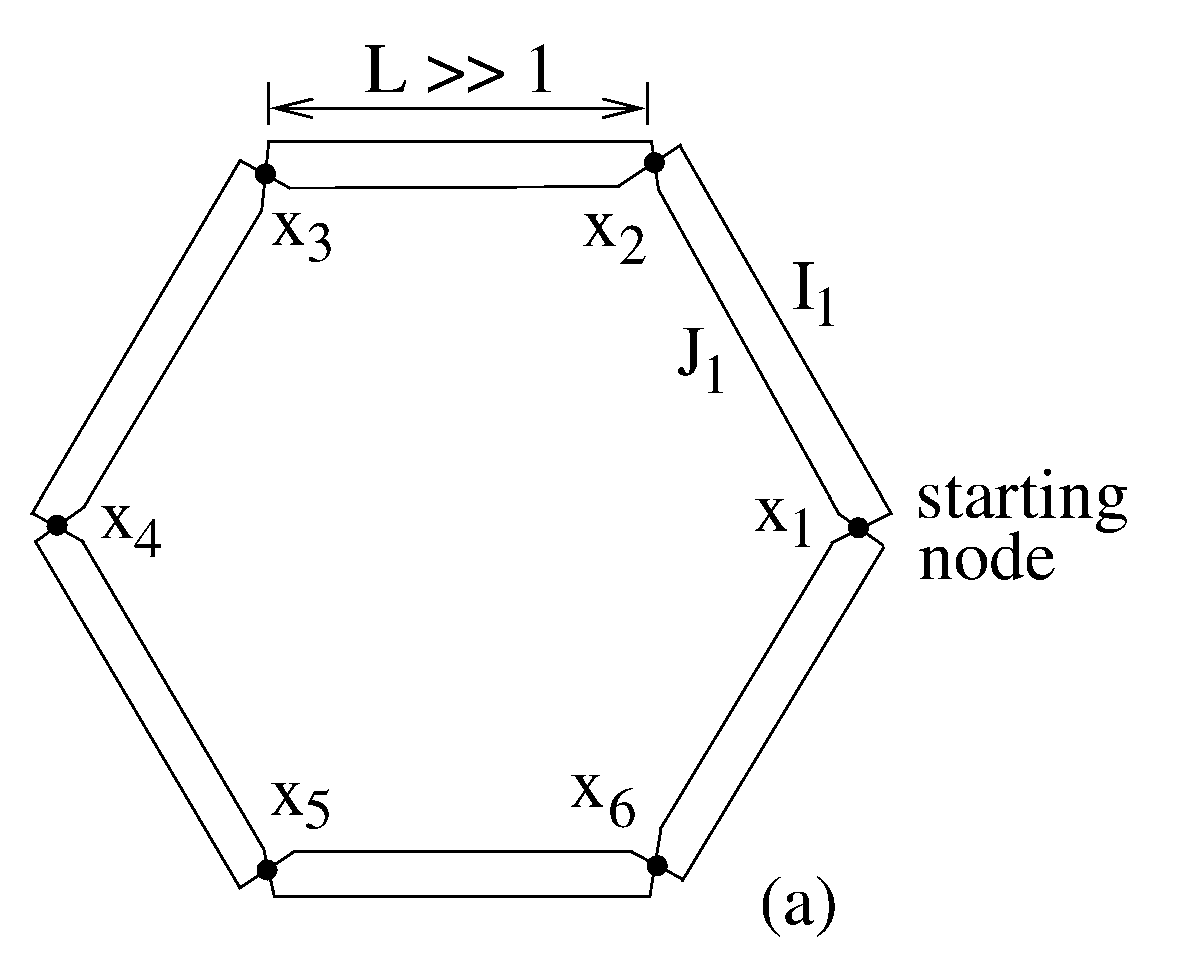
\includegraphics[width=\linewidth]{Images/fig13a.png}
            \caption{Double ring environment.}
        \end{figure}
        \column{0.5\textwidth}
        \begin{itemize}
            \item Lower bound for any online algorithm
            \item W.l.o.g point robot on graph
            \item Detection range $1 - \delta$
            \item Let $x_1, ..., x_k$ nodes of ring (ccw. order)
            \item $I_i$, $J_i$ paralell edges connecting $x_i$ and $x_{i+1}$
            \item $L$ length of $I_i$ and $J_i$
        \end{itemize}
    \end{columns}
\end{frame}


\begin{frame}{Theorem 2}
    \begin{columns}
        \column{0.5\textwidth}
        \begin{figure}
            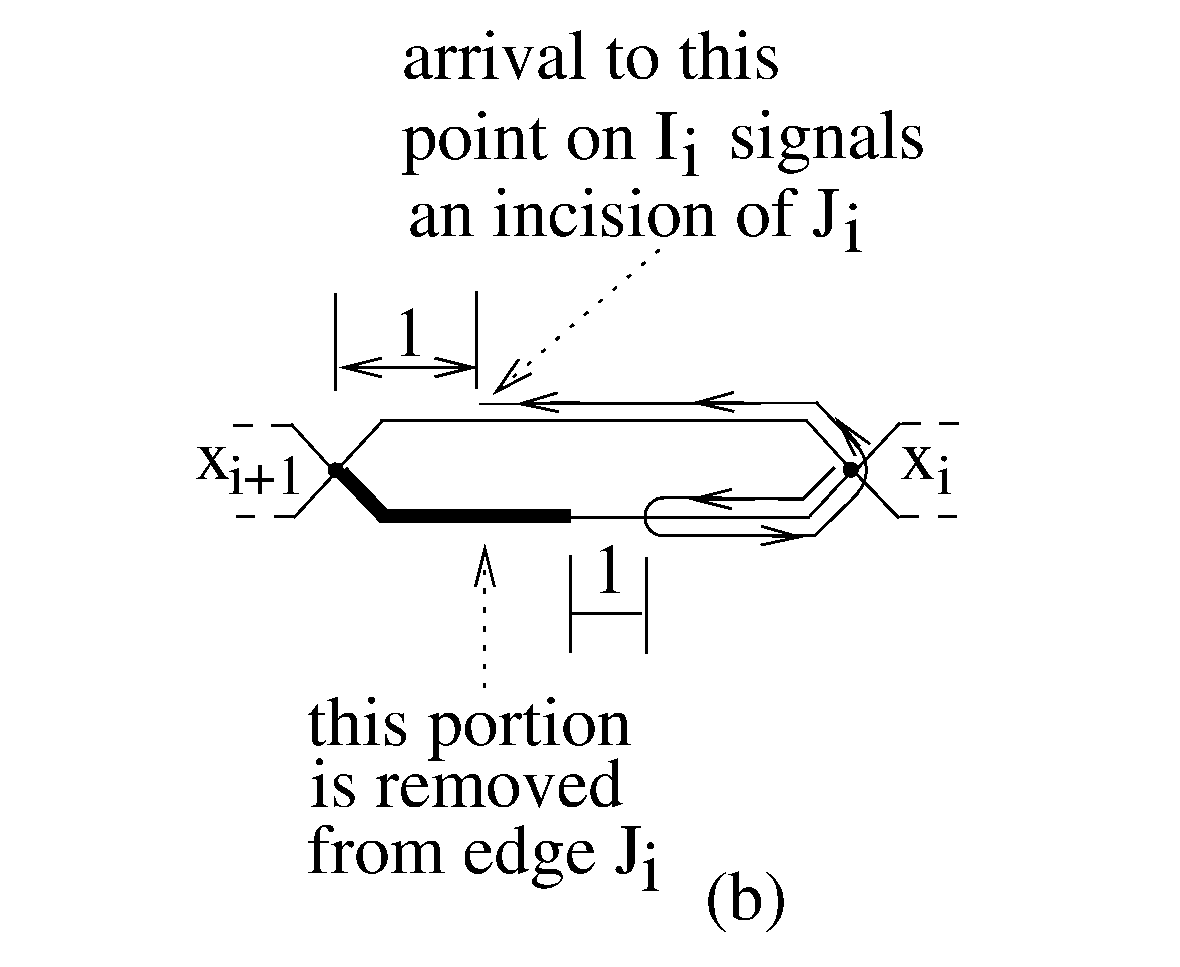
\includegraphics[width=0.8\linewidth]{Images/fig13b.png}
            \caption{Incision procedure}
        \end{figure}
        \column{0.5\textwidth}
        \begin{itemize}
            \item At instant when robot is 1 distance away from $x_{i+1}$ on $I_i$
            \item Truncate $J_i$ at distance 1 of already visited part
            \item $H_i := $ length of $J_i$ that was covered before incision
            \item $H := \sum_{i = 1}^{k} H_i$
            \item Incision special case at starting position
        \end{itemize}
    \end{columns}
\end{frame}

\subsection{Theorem 2}
\begin{frame}{Theorem 2}
    \begin{columns}
        \column{0.5\textwidth}
        \begin{itemize}
            \item Consider best case scenario (say ccw. order)
            \item First Loop: $I_1, ... I_k$ + $2 \cdot H_1, ... 2 \cdot H_k$
            \item Remaining part of $J_1, ... J_k$ covered in second loop
            \item Cost on $I_1, ... I_k$ is: $2kL$
            \item Cost on $J_1, ... J_k$ is: $2H$ in first round
            \item And $2(H + k)$ in second round
        \end{itemize}
        \column{0.5\textwidth}
        \begin{figure}
            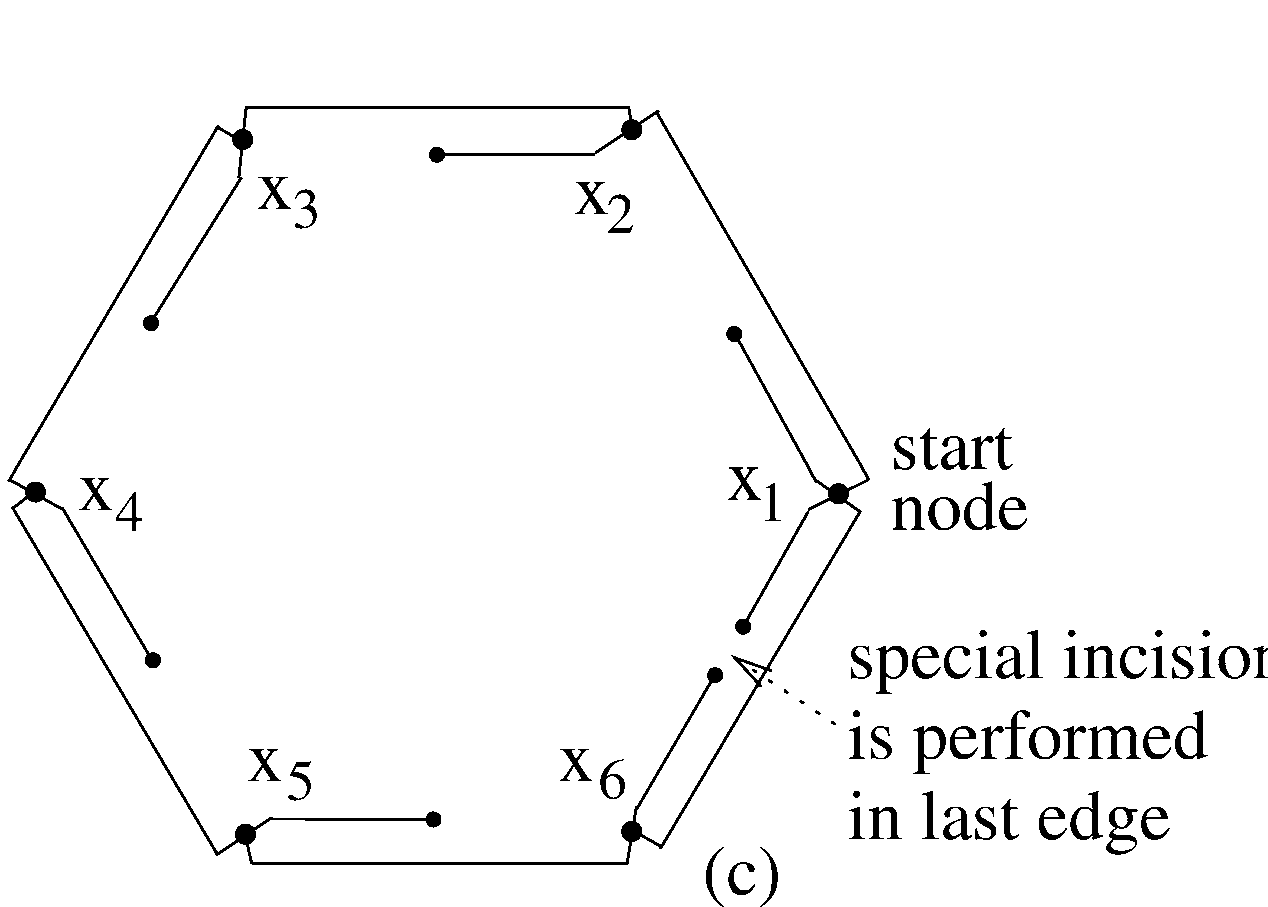
\includegraphics[width=\linewidth]{Images/fig13c.png}
            \caption{Incisions in double ring environment.}
        \end{figure}
    \end{columns}
\end{frame}

\begin{frame}{Theorem 2}
    \begin{proof}
        \begin{itemize}
            \item Online Lower Bound: $l_{\mathcal{A}} \geq 2kL + 4H + 2k$
            \item Offline Upper Bound: $l_{opt} \leq kL + 2(H + k)$
            \item $\implies l_{\mathcal{A}} \geq (2 - \epsilon) l_{opt}$ where $\epsilon = \frac{2k}{kL + 2(H + k)} \ll 1$ as $L \gg 1$
        \end{itemize}
    \end{proof}
\end{frame}

\section{Conclusion}
\begin{frame}{Conclusion}
    \begin{itemize}
        \item Spiral STC and Scan STC are $2 - \epsilon$ competitive online algorithms for the coverage problem
        \item In practice, where $m \ll n$ the algorithms are close to optimal (comp. ratio $2 - \epsilon$ and $\epsilon$ approaches 1)
        \item Online Algorithm can not get better than $2 - \epsilon$ competitive
        \item Spiral STC and Scan STC are optimal online algorithms
    \end{itemize}
\end{frame}

\begin{frame}[focus]
    Thanks!
\end{frame}

%----------------------------------------------------------------------------------------
%	 CLOSING/SUPPLEMENTARY SLIDES
%----------------------------------------------------------------------------------------

\appendix

\begin{frame}{References}
    \nocite{*} % Display all references regardless of if they were cited
    \bibliography{bibliography.bib}
    \bibliographystyle{plain}
\end{frame}

\subsection{Optimality and Competitive Ratio - Details}
\begin{frame}{Optimality and Competitive Ratio - Details}
    \begin{itemize}
        \item Area of grid: $A := n \cdot D^2$
        \item Area of boundary cells: $\delta A := m \cdot D^2$
        \item $l_{opt} \geq \frac{A}{D} = \frac{nD^2}{D} = n \cdot D$
        \item $l_{stc} \leq (n + m) \cdot D$
    \end{itemize}

    $$ \frac{l_{stc}}{l_{opt}} \leq \frac{(n+m) \cdot D}{n \cdot D} = \frac{(n + m) D^2}{n D^2} = \frac{nD^2 + mD^2}{nD^2} = \frac{nD^2 \cdot (1 + \frac{mD^2}{nD^2})}{nD^2}$$
    $$= 1 + \frac{mD^2}{nD^2} = 1 + \frac{\delta A}{A} = 2 - \epsilon$$
    with $\epsilon = (1 - \frac{\delta A}{A})$ and $0 \leq \epsilon \leq 1$ as $A \geq \delta A$ and $A, \delta A \geq 0$
\end{frame}
%------------------------------------------------

% \begin{frame}{Backup Slide}
%     This is a backup slide, useful to include additional materials to answer questions from the audience.
%     \vfill
%     The package \texttt{appendixnumberbeamer} is used to refrain from numbering appendix slides.
% \end{frame}

%----------------------------------------------------------------------------------------

\end{document}

%------------------------------------------------

% \begin{frame}{Simple Slide}
%     This is a simple slide.
% \end{frame}

% %------------------------------------------------
% \subsection{Subsection 1}

% \begin{frame}[plain]{Plain Slide}
%     This is a slide with the plain style and it is numbered.
% \end{frame}

% %------------------------------------------------

% \begin{frame}[t]
%     This slide has an empty title and is aligned to top.
% \end{frame}

% %------------------------------------------------

% \begin{frame}[noframenumbering]{No Slide Numbering}
%     This slide is not numbered and is citing reference \cite{knuth74}.
% \end{frame}

% %------------------------------------------------

% \begin{frame}{Typesetting and Math}
%     The packages \texttt{inputenc} and \texttt{FiraSans}\footnote{\url{https://fonts.google.com/specimen/Fira+Sans}}\textsuperscript{,}\footnote{\url{http://mozilla.github.io/Fira/}} are used to properly set the main fonts.
%     \vfill
%     This theme provides styling commands to typeset \emph{emphasized}, \alert{alerted}, \textbf{bold}, \textcolor{example}{example text}, \dots
%     \vfill
%     \texttt{FiraSans} also provides support for mathematical symbols:
%     \begin{equation*}
%         e^{i\pi} + 1 = 0.
%     \end{equation*}
% \end{frame}

%----------------------------------------------------------------------------------------
%	 SECTION 2
%----------------------------------------------------------------------------------------

%------------------------------------------------

% \begin{frame}{Columns}
% 	\begin{columns}
% 		\column{0.5\textwidth}
% 		This text appears in the left column and wraps neatly with a margin between columns.

% 		\column{0.5\textwidth}
% 		
\includegraphics[width=\linewidth]{Images/placeholder.jpg}
% 	\end{columns}
% \end{frame}

%------------------------------------------------

% \begin{frame}{Lists}
% 	\begin{columns}[T, onlytextwidth] % T for top align, onlytextwidth to suppress the margin between columns
% 		\column{0.33\textwidth}
% 		Items:
% 		\begin{itemize}
% 			\item Item 1
% 			      \begin{itemize}
% 				      \item Subitem 1.1
% 				      \item Subitem 1.2
% 			      \end{itemize}
% 			\item Item 2
% 			\item Item 3
% 		\end{itemize}

% 		\column{0.33\textwidth}
% 		Enumerations:
% 		\begin{enumerate}
% 			\item First
% 			\item Second
% 			      \begin{enumerate}
% 				      \item Sub-first
% 				      \item Sub-second
% 			      \end{enumerate}
% 			\item Third
% 		\end{enumerate}

% 		\column{0.33\textwidth}
% 		Descriptions:
% 		\begin{description}
% 			\item[First] Yes.
% 			\item[Second] No.
% 		\end{description}
% 	\end{columns}
% \end{frame}

%------------------------------------------------

% \begin{frame}{Table}
% 	\begin{table}
% 		\centering % Centre the table on the slide
% 		\begin{tabular}{l c}
% 			\toprule
% 			Discipline                           & Avg. Salary       \\
% 			\toprule
% 			\textbf{Engineering}                 & \textbf{\$66,521} \\
% 			Computer Sciences                    & \$60,005          \\
% 			Mathematics and Sciences             & \$61,867          \\
% 			Business                             & \$56,720          \\
% 			Humanities \& Social Sciences        & \$56,669          \\
% 			Agriculture and Natural Resources    & \$53,565          \\
% 			Communications                       & \$51,448          \\
% 			\midrule
% 			\textbf{Average for All Disciplines} & \textbf{\$58,114} \\
% 			\bottomrule
% 		\end{tabular}
% 		\caption{Table caption}
% 	\end{table}
% \end{frame}

%------------------------------------------------
% \begin{frame}{Blocks}
%     These blocks are part of 1 slide, to be displayed consecutively.
%     \begin{block}{Block}
%         Text.
%     \end{block}
%     \pause % Automatically creates a new "page" split between the above and above + below
%     \begin{alertblock}{Alert block}
%         Alert \alert{text}.
%     \end{alertblock}
%     \pause % Automatically creates a new "page" split between the above and above + below
%     \begin{exampleblock}{Example block}
%         Example \textcolor{example}{text}.
%     \end{exampleblock}
% \end{frame}